\documentclass[12pt,a4paper,twoside,openright]{book}

\usepackage[utf8]{inputenc}
\usepackage[italian]{babel}
\usepackage[T1]{fontenc}

\usepackage{style/isi_style_lt}

\usepackage{amsmath,amsfonts,amssymb,amsthm}
\usepackage{caption}
\usepackage[usenames]{color}
\usepackage{enumerate}
\usepackage{fancyhdr}
\usepackage{fancyvrb}
\usepackage{float}
\usepackage{graphicx}
\usepackage{booktabs}
\usepackage{indentfirst}
\usepackage{listings}
\usepackage{marvosym}
\usepackage{multicol}
\usepackage{sectsty}
\usepackage{subcaption}
\usepackage{tocloft}
\usepackage{microtype}
\usepackage[table]{xcolor}
\usepackage{url}
\usepackage{hyperref}
\usepackage{adjustbox}
\usepackage{tikz}
\usetikzlibrary{positioning}


    \usepackage{adjustbox} % Used to constrain images to a maximum size 
    \usepackage{textcomp} % defines textquotesingle
    % Hack from http://tex.stackexchange.com/a/47451/13684:
    \AtBeginDocument{%
        \def\PYZsq{\textquotesingle}% Upright quotes in Pygmentized code
    }
    \usepackage{upquote} % Upright quotes for verbatim code
    \usepackage{eurosym} % defines \euro
    \usepackage[mathletters]{ucs} % Extended unicode (utf-8) support
    \usepackage{grffile} % extends the file name processing of package graphics 
                         % to support a larger range 
    \usepackage{longtable} % longtable support required by pandoc >1.10
    \usepackage{booktabs}  % table support for pandoc > 1.12.2
    \usepackage[inline]{enumitem} % IRkernel/repr support (it uses the enumerate* environment)
    \usepackage[normalem]{ulem} % ulem is needed to support strikethroughs (\sout)

    
    % Colors for the hyperref package
    \definecolor{urlcolor}{rgb}{0,.145,.698}
    \definecolor{linkcolor}{rgb}{.71,0.21,0.01}
    \definecolor{citecolor}{rgb}{.12,.54,.11}

    % ANSI colors
    \definecolor{ansi-black}{HTML}{3E424D}
    \definecolor{ansi-black-intense}{HTML}{282C36}
    \definecolor{ansi-red}{HTML}{E75C58}
    \definecolor{ansi-red-intense}{HTML}{B22B31}
    \definecolor{ansi-green}{HTML}{00A250}
    \definecolor{ansi-green-intense}{HTML}{007427}
    \definecolor{ansi-yellow}{HTML}{DDB62B}
    \definecolor{ansi-yellow-intense}{HTML}{B27D12}
    \definecolor{ansi-blue}{HTML}{208FFB}
    \definecolor{ansi-blue-intense}{HTML}{0065CA}
    \definecolor{ansi-magenta}{HTML}{D160C4}
    \definecolor{ansi-magenta-intense}{HTML}{A03196}
    \definecolor{ansi-cyan}{HTML}{60C6C8}
    \definecolor{ansi-cyan-intense}{HTML}{258F8F}
    \definecolor{ansi-white}{HTML}{C5C1B4}
    \definecolor{ansi-white-intense}{HTML}{A1A6B2}

    % commands and environments needed by pandoc snippets
    % extracted from the output of `pandoc -s`
    \providecommand{\tightlist}{%
      \setlength{\itemsep}{0pt}\setlength{\parskip}{0pt}}
    \DefineVerbatimEnvironment{Highlighting}{Verbatim}{commandchars=\\\{\}}
    % Add ',fontsize=\small' for more characters per line
    \newenvironment{Shaded}{}{}
    \newcommand{\KeywordTok}[1]{\textcolor[rgb]{0.00,0.44,0.13}{\textbf{{#1}}}}
    \newcommand{\DataTypeTok}[1]{\textcolor[rgb]{0.56,0.13,0.00}{{#1}}}
    \newcommand{\DecValTok}[1]{\textcolor[rgb]{0.25,0.63,0.44}{{#1}}}
    \newcommand{\BaseNTok}[1]{\textcolor[rgb]{0.25,0.63,0.44}{{#1}}}
    \newcommand{\FloatTok}[1]{\textcolor[rgb]{0.25,0.63,0.44}{{#1}}}
    \newcommand{\CharTok}[1]{\textcolor[rgb]{0.25,0.44,0.63}{{#1}}}
    \newcommand{\StringTok}[1]{\textcolor[rgb]{0.25,0.44,0.63}{{#1}}}
    \newcommand{\CommentTok}[1]{\textcolor[rgb]{0.38,0.63,0.69}{\textit{{#1}}}}
    \newcommand{\OtherTok}[1]{\textcolor[rgb]{0.00,0.44,0.13}{{#1}}}
    \newcommand{\AlertTok}[1]{\textcolor[rgb]{1.00,0.00,0.00}{\textbf{{#1}}}}
    \newcommand{\FunctionTok}[1]{\textcolor[rgb]{0.02,0.16,0.49}{{#1}}}
    \newcommand{\RegionMarkerTok}[1]{{#1}}
    \newcommand{\ErrorTok}[1]{\textcolor[rgb]{1.00,0.00,0.00}{\textbf{{#1}}}}
    \newcommand{\NormalTok}[1]{{#1}}
    
    % Additional commands for more recent versions of Pandoc
    \newcommand{\ConstantTok}[1]{\textcolor[rgb]{0.53,0.00,0.00}{{#1}}}
    \newcommand{\SpecialCharTok}[1]{\textcolor[rgb]{0.25,0.44,0.63}{{#1}}}
    \newcommand{\VerbatimStringTok}[1]{\textcolor[rgb]{0.25,0.44,0.63}{{#1}}}
    \newcommand{\SpecialStringTok}[1]{\textcolor[rgb]{0.73,0.40,0.53}{{#1}}}
    \newcommand{\ImportTok}[1]{{#1}}
    \newcommand{\DocumentationTok}[1]{\textcolor[rgb]{0.73,0.13,0.13}{\textit{{#1}}}}
    \newcommand{\AnnotationTok}[1]{\textcolor[rgb]{0.38,0.63,0.69}{\textbf{\textit{{#1}}}}}
    \newcommand{\CommentVarTok}[1]{\textcolor[rgb]{0.38,0.63,0.69}{\textbf{\textit{{#1}}}}}
    \newcommand{\VariableTok}[1]{\textcolor[rgb]{0.10,0.09,0.49}{{#1}}}
    \newcommand{\ControlFlowTok}[1]{\textcolor[rgb]{0.00,0.44,0.13}{\textbf{{#1}}}}
    \newcommand{\OperatorTok}[1]{\textcolor[rgb]{0.40,0.40,0.40}{{#1}}}
    \newcommand{\BuiltInTok}[1]{{#1}}
    \newcommand{\ExtensionTok}[1]{{#1}}
    \newcommand{\PreprocessorTok}[1]{\textcolor[rgb]{0.74,0.48,0.00}{{#1}}}
    \newcommand{\AttributeTok}[1]{\textcolor[rgb]{0.49,0.56,0.16}{{#1}}}
    \newcommand{\InformationTok}[1]{\textcolor[rgb]{0.38,0.63,0.69}{\textbf{\textit{{#1}}}}}
    \newcommand{\WarningTok}[1]{\textcolor[rgb]{0.38,0.63,0.69}{\textbf{\textit{{#1}}}}}
    
    
    % Define a nice break command that doesn't care if a line doesn't already
    % exist.
    \def\br{\hspace*{\fill} \\* }
    % Math Jax compatability definitions
    \def\gt{>}
    \def\lt{<}
    % Document parameters
    \title{Untitled1}
    
    
    

    % Pygments definitions
    
\makeatletter
\def\PY@reset{\let\PY@it=\relax \let\PY@bf=\relax%
    \let\PY@ul=\relax \let\PY@tc=\relax%
    \let\PY@bc=\relax \let\PY@ff=\relax}
\def\PY@tok#1{\csname PY@tok@#1\endcsname}
\def\PY@toks#1+{\ifx\relax#1\empty\else%
    \PY@tok{#1}\expandafter\PY@toks\fi}
\def\PY@do#1{\PY@bc{\PY@tc{\PY@ul{%
    \PY@it{\PY@bf{\PY@ff{#1}}}}}}}
\def\PY#1#2{\PY@reset\PY@toks#1+\relax+\PY@do{#2}}

\expandafter\def\csname PY@tok@w\endcsname{\def\PY@tc##1{\textcolor[rgb]{0.73,0.73,0.73}{##1}}}
\expandafter\def\csname PY@tok@c\endcsname{\let\PY@it=\textit\def\PY@tc##1{\textcolor[rgb]{0.25,0.50,0.50}{##1}}}
\expandafter\def\csname PY@tok@cp\endcsname{\def\PY@tc##1{\textcolor[rgb]{0.74,0.48,0.00}{##1}}}
\expandafter\def\csname PY@tok@k\endcsname{\let\PY@bf=\textbf\def\PY@tc##1{\textcolor[rgb]{0.00,0.50,0.00}{##1}}}
\expandafter\def\csname PY@tok@kp\endcsname{\def\PY@tc##1{\textcolor[rgb]{0.00,0.50,0.00}{##1}}}
\expandafter\def\csname PY@tok@kt\endcsname{\def\PY@tc##1{\textcolor[rgb]{0.69,0.00,0.25}{##1}}}
\expandafter\def\csname PY@tok@o\endcsname{\def\PY@tc##1{\textcolor[rgb]{0.40,0.40,0.40}{##1}}}
\expandafter\def\csname PY@tok@ow\endcsname{\let\PY@bf=\textbf\def\PY@tc##1{\textcolor[rgb]{0.67,0.13,1.00}{##1}}}
\expandafter\def\csname PY@tok@nb\endcsname{\def\PY@tc##1{\textcolor[rgb]{0.00,0.50,0.00}{##1}}}
\expandafter\def\csname PY@tok@nf\endcsname{\def\PY@tc##1{\textcolor[rgb]{0.00,0.00,1.00}{##1}}}
\expandafter\def\csname PY@tok@nc\endcsname{\let\PY@bf=\textbf\def\PY@tc##1{\textcolor[rgb]{0.00,0.00,1.00}{##1}}}
\expandafter\def\csname PY@tok@nn\endcsname{\let\PY@bf=\textbf\def\PY@tc##1{\textcolor[rgb]{0.00,0.00,1.00}{##1}}}
\expandafter\def\csname PY@tok@ne\endcsname{\let\PY@bf=\textbf\def\PY@tc##1{\textcolor[rgb]{0.82,0.25,0.23}{##1}}}
\expandafter\def\csname PY@tok@nv\endcsname{\def\PY@tc##1{\textcolor[rgb]{0.10,0.09,0.49}{##1}}}
\expandafter\def\csname PY@tok@no\endcsname{\def\PY@tc##1{\textcolor[rgb]{0.53,0.00,0.00}{##1}}}
\expandafter\def\csname PY@tok@nl\endcsname{\def\PY@tc##1{\textcolor[rgb]{0.63,0.63,0.00}{##1}}}
\expandafter\def\csname PY@tok@ni\endcsname{\let\PY@bf=\textbf\def\PY@tc##1{\textcolor[rgb]{0.60,0.60,0.60}{##1}}}
\expandafter\def\csname PY@tok@na\endcsname{\def\PY@tc##1{\textcolor[rgb]{0.49,0.56,0.16}{##1}}}
\expandafter\def\csname PY@tok@nt\endcsname{\let\PY@bf=\textbf\def\PY@tc##1{\textcolor[rgb]{0.00,0.50,0.00}{##1}}}
\expandafter\def\csname PY@tok@nd\endcsname{\def\PY@tc##1{\textcolor[rgb]{0.67,0.13,1.00}{##1}}}
\expandafter\def\csname PY@tok@s\endcsname{\def\PY@tc##1{\textcolor[rgb]{0.73,0.13,0.13}{##1}}}
\expandafter\def\csname PY@tok@sd\endcsname{\let\PY@it=\textit\def\PY@tc##1{\textcolor[rgb]{0.73,0.13,0.13}{##1}}}
\expandafter\def\csname PY@tok@si\endcsname{\let\PY@bf=\textbf\def\PY@tc##1{\textcolor[rgb]{0.73,0.40,0.53}{##1}}}
\expandafter\def\csname PY@tok@se\endcsname{\let\PY@bf=\textbf\def\PY@tc##1{\textcolor[rgb]{0.73,0.40,0.13}{##1}}}
\expandafter\def\csname PY@tok@sr\endcsname{\def\PY@tc##1{\textcolor[rgb]{0.73,0.40,0.53}{##1}}}
\expandafter\def\csname PY@tok@ss\endcsname{\def\PY@tc##1{\textcolor[rgb]{0.10,0.09,0.49}{##1}}}
\expandafter\def\csname PY@tok@sx\endcsname{\def\PY@tc##1{\textcolor[rgb]{0.00,0.50,0.00}{##1}}}
\expandafter\def\csname PY@tok@m\endcsname{\def\PY@tc##1{\textcolor[rgb]{0.40,0.40,0.40}{##1}}}
\expandafter\def\csname PY@tok@gh\endcsname{\let\PY@bf=\textbf\def\PY@tc##1{\textcolor[rgb]{0.00,0.00,0.50}{##1}}}
\expandafter\def\csname PY@tok@gu\endcsname{\let\PY@bf=\textbf\def\PY@tc##1{\textcolor[rgb]{0.50,0.00,0.50}{##1}}}
\expandafter\def\csname PY@tok@gd\endcsname{\def\PY@tc##1{\textcolor[rgb]{0.63,0.00,0.00}{##1}}}
\expandafter\def\csname PY@tok@gi\endcsname{\def\PY@tc##1{\textcolor[rgb]{0.00,0.63,0.00}{##1}}}
\expandafter\def\csname PY@tok@gr\endcsname{\def\PY@tc##1{\textcolor[rgb]{1.00,0.00,0.00}{##1}}}
\expandafter\def\csname PY@tok@ge\endcsname{\let\PY@it=\textit}
\expandafter\def\csname PY@tok@gs\endcsname{\let\PY@bf=\textbf}
\expandafter\def\csname PY@tok@gp\endcsname{\let\PY@bf=\textbf\def\PY@tc##1{\textcolor[rgb]{0.00,0.00,0.50}{##1}}}
\expandafter\def\csname PY@tok@go\endcsname{\def\PY@tc##1{\textcolor[rgb]{0.53,0.53,0.53}{##1}}}
\expandafter\def\csname PY@tok@gt\endcsname{\def\PY@tc##1{\textcolor[rgb]{0.00,0.27,0.87}{##1}}}
\expandafter\def\csname PY@tok@err\endcsname{\def\PY@bc##1{\setlength{\fboxsep}{0pt}\fcolorbox[rgb]{1.00,0.00,0.00}{1,1,1}{\strut ##1}}}
\expandafter\def\csname PY@tok@kc\endcsname{\let\PY@bf=\textbf\def\PY@tc##1{\textcolor[rgb]{0.00,0.50,0.00}{##1}}}
\expandafter\def\csname PY@tok@kd\endcsname{\let\PY@bf=\textbf\def\PY@tc##1{\textcolor[rgb]{0.00,0.50,0.00}{##1}}}
\expandafter\def\csname PY@tok@kn\endcsname{\let\PY@bf=\textbf\def\PY@tc##1{\textcolor[rgb]{0.00,0.50,0.00}{##1}}}
\expandafter\def\csname PY@tok@kr\endcsname{\let\PY@bf=\textbf\def\PY@tc##1{\textcolor[rgb]{0.00,0.50,0.00}{##1}}}
\expandafter\def\csname PY@tok@bp\endcsname{\def\PY@tc##1{\textcolor[rgb]{0.00,0.50,0.00}{##1}}}
\expandafter\def\csname PY@tok@fm\endcsname{\def\PY@tc##1{\textcolor[rgb]{0.00,0.00,1.00}{##1}}}
\expandafter\def\csname PY@tok@vc\endcsname{\def\PY@tc##1{\textcolor[rgb]{0.10,0.09,0.49}{##1}}}
\expandafter\def\csname PY@tok@vg\endcsname{\def\PY@tc##1{\textcolor[rgb]{0.10,0.09,0.49}{##1}}}
\expandafter\def\csname PY@tok@vi\endcsname{\def\PY@tc##1{\textcolor[rgb]{0.10,0.09,0.49}{##1}}}
\expandafter\def\csname PY@tok@vm\endcsname{\def\PY@tc##1{\textcolor[rgb]{0.10,0.09,0.49}{##1}}}
\expandafter\def\csname PY@tok@sa\endcsname{\def\PY@tc##1{\textcolor[rgb]{0.73,0.13,0.13}{##1}}}
\expandafter\def\csname PY@tok@sb\endcsname{\def\PY@tc##1{\textcolor[rgb]{0.73,0.13,0.13}{##1}}}
\expandafter\def\csname PY@tok@sc\endcsname{\def\PY@tc##1{\textcolor[rgb]{0.73,0.13,0.13}{##1}}}
\expandafter\def\csname PY@tok@dl\endcsname{\def\PY@tc##1{\textcolor[rgb]{0.73,0.13,0.13}{##1}}}
\expandafter\def\csname PY@tok@s2\endcsname{\def\PY@tc##1{\textcolor[rgb]{0.73,0.13,0.13}{##1}}}
\expandafter\def\csname PY@tok@sh\endcsname{\def\PY@tc##1{\textcolor[rgb]{0.73,0.13,0.13}{##1}}}
\expandafter\def\csname PY@tok@s1\endcsname{\def\PY@tc##1{\textcolor[rgb]{0.73,0.13,0.13}{##1}}}
\expandafter\def\csname PY@tok@mb\endcsname{\def\PY@tc##1{\textcolor[rgb]{0.40,0.40,0.40}{##1}}}
\expandafter\def\csname PY@tok@mf\endcsname{\def\PY@tc##1{\textcolor[rgb]{0.40,0.40,0.40}{##1}}}
\expandafter\def\csname PY@tok@mh\endcsname{\def\PY@tc##1{\textcolor[rgb]{0.40,0.40,0.40}{##1}}}
\expandafter\def\csname PY@tok@mi\endcsname{\def\PY@tc##1{\textcolor[rgb]{0.40,0.40,0.40}{##1}}}
\expandafter\def\csname PY@tok@il\endcsname{\def\PY@tc##1{\textcolor[rgb]{0.40,0.40,0.40}{##1}}}
\expandafter\def\csname PY@tok@mo\endcsname{\def\PY@tc##1{\textcolor[rgb]{0.40,0.40,0.40}{##1}}}
\expandafter\def\csname PY@tok@ch\endcsname{\let\PY@it=\textit\def\PY@tc##1{\textcolor[rgb]{0.25,0.50,0.50}{##1}}}
\expandafter\def\csname PY@tok@cm\endcsname{\let\PY@it=\textit\def\PY@tc##1{\textcolor[rgb]{0.25,0.50,0.50}{##1}}}
\expandafter\def\csname PY@tok@cpf\endcsname{\let\PY@it=\textit\def\PY@tc##1{\textcolor[rgb]{0.25,0.50,0.50}{##1}}}
\expandafter\def\csname PY@tok@c1\endcsname{\let\PY@it=\textit\def\PY@tc##1{\textcolor[rgb]{0.25,0.50,0.50}{##1}}}
\expandafter\def\csname PY@tok@cs\endcsname{\let\PY@it=\textit\def\PY@tc##1{\textcolor[rgb]{0.25,0.50,0.50}{##1}}}

\def\PYZbs{\char`\\}
\def\PYZus{\char`\_}
\def\PYZob{\char`\{}
\def\PYZcb{\char`\}}
\def\PYZca{\char`\^}
\def\PYZam{\char`\&}
\def\PYZlt{\char`\<}
\def\PYZgt{\char`\>}
\def\PYZsh{\char`\#}
\def\PYZpc{\char`\%}
\def\PYZdl{\char`\$}
\def\PYZhy{\char`\-}
\def\PYZsq{\char`\'}
\def\PYZdq{\char`\"}
\def\PYZti{\char`\~}
% for compatibility with earlier versions
\def\PYZat{@}
\def\PYZlb{[}
\def\PYZrb{]}
\makeatother


    % Exact colors from NB
    \definecolor{incolor}{rgb}{0.0, 0.0, 0.5}
    \definecolor{outcolor}{rgb}{0.545, 0.0, 0.0}




\hypersetup{%
	pdfpagemode={UseOutlines},
	bookmarksopen,
	pdfstartview={FitH},
	colorlinks,
	linkcolor={black},
	citecolor={black},
	urlcolor={black}
}

\AtBeginDocument{%
	\renewcommand{\contentsname}{Indice}
	\renewcommand\tablename{Tabella}
	\renewcommand\figurename{Figura}
	\renewcommand{\lstlistingname}{Listato}
	\renewcommand{\refname}{Riferimenti}
}

\definecolor{dkgreen}{rgb}{0,0.6,0}
\definecolor{gray}{rgb}{0.5,0.5,0.5}
\definecolor{mauve}{rgb}{0.58,0,0.82}
\definecolor{bracecolor}{rgb}{1, 0.788, 0.133}
\definecolor{keywordcolor}{rgb}{0.773, 0.376, 0.408}
\definecolor{stringcolor}{rgb}{0.780, 0.537, 0.839}
\definecolor{punct}{rgb}{0.0, 0.0, 0.0}
\definecolor{darkblue}{rgb}{0.0,0.0,0.6}
\definecolor{lightblue}{rgb}{0.0,0.0,0.9}
\definecolor{cyan}{rgb}{0.0,0.6,0.6}
\definecolor{darkred}{rgb}{0.6,0.0,0.0}

\definecolor{framecolor}{gray}{0.4} % Define the color for the frame

\DeclareFloatingEnvironment[
    fileext=loc,
    listname={List of Codes},
    name=Listato,
]{customcode}

\DeclareTCBListing{mintedbox}{O{}m!O{}}{
  listing engine=minted,
  listing only,
  minted language=#2,
  minted style=default,
  minted options={
    gobble=0,
    breaklines=true,
    breakafter=,,
    fontsize=\scriptsize,
    linenos,  
    #1},
  boxsep=3pt,
  left=3pt,
  right=3pt,
  top=3pt,
  bottom=3pt,
  arc=0pt,
  leftrule=0pt,
  rightrule=0pt,
  bottomrule=0pt,
  toprule=0pt,
  colback=white,
  colframe=framecolor,
  coltext=black,
  boxrule=0.5pt,
  overlay={},
  #3
}



\makeatletter
\def\cleardoublepage{
	\clearpage\if@twoside \ifodd\c@page\else
	\hbox{}
	\thispagestyle{empty}
	\newpage
	\if@twocolumn\hbox{}\newpage\fi\fi\fi
}

\makeatother

\setlength{\textwidth}{14cm}
\setlength{\textheight}{21cm}
\setlength{\footskip}{3cm}

\setlength{\hoffset}{0pt}
\setlength{\voffset}{0pt}

\setlength{\oddsidemargin}{1cm}
\setlength{\evensidemargin}{1cm}

\universita{Alma Mater Studiorum -- Università di Bologna}

\campus{Campus di Cesena}

\scuola{Scuola di Scienze}

\corsodilaurea{Corso di Laurea in Ingegneria e Scienze Informatiche}

\titolo{SciLay: Un Nuovo Dataset per Long Document Abstractive Summarization Tecnica e Lay di Articoli Biomedici}

\materia{Programmazione Di Applicazioni Data Intensive}

\laureando{Mattia Panni}

\relatore[Prof.]{Gianluca Moro}
\correlatoreA[Ing.]{Paolo Italiani}
\correlatoreB[Ing.]{Luca Ragazzi}

\sessione{Seconda} 

\annoaccademico{2022 -- 2023}

\parolechiave 
{Summarization}
{Natural Language Processing}
{Machine Learning}
{Deep Neural Networks}
{Seq2Seq Models}



\dedica{\emph{Il problema non è l'ascesa delle macchine ``intelligenti'', \\
                ma l'instupidimento dell'umanità.}\cite{books/gigerenzer/intelligenza}}

\makeindex

\begin{document}

\frontmatter 

\maketitle

\chapter*{Introduzione}
\markboth{Introduzione}{Introduzione}


L'\emph{intelligenza artificiale} (AI) è un campo interdisciplinare che si concentra sulla creazione di sistemi o macchine in grado di eseguire attività che richiedono, fra le altre cose

\begin{itemize}
    \item \textbf{Apprendimento automatico}. Le AI utilizzano tecniche di apprendimento automatico per acquisire conoscenze dai dati. Questo significa che anziché essere programmate esplicitamente per eseguire compiti specifici, come accade per gli algoritmi tradizionali, le AI apprendono dai dati e migliorano le loro prestazioni con l'esperienza. 
    \item \textbf{Generalizzazione}. Le AI sono in grado di adattarsi a nuove situazioni e compiti. Possono generalizzare le loro conoscenze per risolvere problemi simili a quelli affrontati durante l'addestramento. 
    \item \textbf{Processamento dei dati non strutturati}: Le AI sono spesso utilizzate per analizzare e comprendere dati non strutturati, come testo, immagini e suoni. Possono estrarre informazioni significative da fonti di dati complesse e rumorose.
\end{itemize}

Queste proprietà, auspicabili per tali sistemi, sono comunemente riconosciute come indicatori di intelligenza, da cui deriva il termine ``Intelligenza Artificiale''.

Questo campo è stato oggetto di ricerca e sviluppo fin dagli anni '50 ed è cresciuto enormemente in importanza e complessità. L'AI ha rivoluzionato molti aspetti della nostra vita, dai motori di ricerca online alla guida autonoma, dalla diagnosi medica all'automazione industriale. 


L'idea di creare macchine che possano simulare l'intelligenza umana ha radici antiche, ma il campo dell'AI moderna è iniziato nel 1956 con una conferenza tenuta a Dartmouth College, dove i ricercatori hanno discusso di ``programmare un computer per simulare l'intelligenza umana''. Questo evento è spesso considerato l'inizio ufficiale dell'AI come campo di studio.

Negli anni '50 e '60, gli studiosi dell'AI erano ottimisti riguardo alle potenzialità della disciplina. Credevano che sarebbe stato relativamente semplice programmare un computer per eseguire compiti che richiedevano intelligenza, come giocare a scacchi o tradurre lingue. Tuttavia, presto divenne chiaro che molte delle attività che gli esseri umani eseguono con facilità sono estremamente complesse da programmare.

Questo ha portato a un periodo noto come ``inverno dell'AI'' negli anni '70 e '80, durante il quale il finanziamento e l'interesse per l'AI diminuirono notevolmente. Ma negli anni '90, con l'aumento della potenza di calcolo, lo sviluppo di nuove tecniche e la disponibilità sempre maggiore di dati, l'AI ha conosciuto una rinascita. Oggi, l'AI è uno dei campi di ricerca e sviluppo più attivi al mondo.



D'altrocanto, come accade per ogni cosa, questo tipo di sistemi ottengono grandi risultati per un certo tipo di problemi, ma non per altri. Quando l'ambiente è stabile, ovvero presenta regole e/o pattern fissi (come nel caso degli scacchi), le AI eguagliano se non addirittura battono le performance degli esseri umani. Tuttavia, in situazioni colme di incertezza, potenza di calcolo elevata e disponibilità di grandi moli di dati contribuiscono in maniera limitata. In altre parole, al verificarsi di ``Cigni neri''\cite{books/taleb/cigno}, ovvero situazioni altamente improbabili ma altrettanto impattanti delle quali, per loro natura, non disponiamo dati, le AI sono ``fragili'', ossia vengono danneggiate da tali eventi.
Il termine ``Cigno nero'' è stato coniato per mettere in evidenza la nostra tendenza a sottovalutare eventi rari ma estremamente influenti e il nostro desiderio retrospettivo di spiegare tali eventi come se fossero stati prevedibili in anticipo. Abbiamo piuttosto ``[...] bisogno di uno sguardo e di un coraggio che ci permettano di rimanere intelligenti in un mondo intelligente''\cite{books/gigerenzer/intelligenza}, da qui la dedica di questo lavoro. 
``Non è tempo di metterci comodi e rilassarci[...]''\cite{books/gigerenzer/intelligenza}, occorre piuttosto comprendere e gestire il rischio associato a tali eventi, piuttosto che presumere che le AI possano prevederli o gestirli autonomamente.

Negli ultimi tempi, il \emph{Machine Learning} (ML) è emerso come una macro-area tecnica di primaria importanza nell'ambito dell'AI. Le sue applicazioni di successo spaziano in diversi settori, tra cui il riconoscimento vocale e la visione artificiale.

Tuttavia, l'efficacia del machine learning può risultare limitata quando si affrontano dati complessi come immagini o testi in linguaggio naturale. La preparazione dei dati e la selezione delle variabili rilevanti richiedono spesso l'intervento di esperti e un notevole sforzo. In queste circostanze, il \emph{Deep Learning} (DP) si è rivelato una risorsa preziosa. Questo approccio è in grado di estrarre autonomamente le variabili più importanti direttamente dai dati grezzi, aprendo nuove prospettive di ricerca.

Il deep learning è un campo relativamente giovane, con potenzialità ancora inesplorate, in grado di eseguire analisi dei dati a un livello più profondo.
L'applicazione del deep learning ha portato a miglioramenti significativi in numerosi settori. Ha reso possibile lo sviluppo di auto a guida autonoma, assistenti virtuali capaci di comprensione del linguaggio naturale e macchinari medici in grado di identificare masse tumorali con una precisione superiore a quella umana.


Entrambe le macro-aree sono figlie dell'enorme impulso derivato dall'analisi dei dati e dalla capacità di estrarre conoscenza da voluminose masse di informazioni. In questo contesto, la disponibilità di dati è diventata cruciale, e l'abbondanza di dati ha reso possibile l'estrazione di conoscenze estremamente precise.

Questo cambiamento è stato alimentato dalla crescente generazione di dati, che avanza con una velocità precedentemente inimmaginabile. Questo scenario ha portato alla necessità di sviluppare i nuovi metodi citati in precedenza, per gestire e analizzare dati le cui dimensioni superano ampiamente le capacità umane.

All'interno di questo lavoro, verranno analizzati e sperimentati diversi approcci recenti nel campo del \emph{Natural Language Processing} (NLP) e del Deep Learning.

Il NLP è una delle sfide più complesse in questo ambito, poiché richiede l'analisi lessicale e semantica del testo scritto. Negli ultimi anni, la ricerca in questo settore ha visto una crescente attenzione, soprattutto a causa della diffusione di dati testuali non strutturati. Tuttavia, questo tipo di dati presenta ambiguità e problematiche, che saranno analizzate in dettaglio.

La tesi si propone di valutare e confrontare vari metodi NLP e DL, evidenziando i loro vantaggi e svantaggi nell'ambito della sfida di estrarre conoscenze comprensibili dal pubblico da articoli scientifici biomedici.
Per fare questo viene presentato un nuovo dataset \emph{SciLay} creato ad'hoc per questo task.

Il lavoro di tesi è stato suddiviso nei seguenti capitoli:

\begin{itemize}
    \item \textbf{Capitolo 1} - Analisi preliminare sulla struttura e modalità di raccolta dei dati.
    \item \textbf{Capitolo 2} - Panoramica sulle varie tecnologie esistenti in letteratura utilizzabili per il problema posto.
    \item \textbf{Capitolo 3} - Introduzione alla modellazione del problema con i primi approcci alle difficoltà riscontrate e alle relative soluzioni.
    \item \textbf{Capitolo 4} - Metodi di risoluzione dei problemi riscontrati e spiegazione dei diversi approcci utilizzati.
    \item \textbf{Capitolo 5} - Il lavoro realizzato e il codice impiegato.
\end{itemize}

\newpage

\tableofcontents

\newpage

\listoffigures

\mainmatter

\pagestyle{fancy} 
\fancyhead[LO]{\nouppercase{\rightmark}}
\fancyhead[RE]{\nouppercase{\leftmark}}
\fancyhead[LE,RO]{\thepage}
\fancyfoot{}


%% CAPITOLO 1

\chapter{Analisi dei dati raccolti}

Questo capitolo tratterà in maniera preliminare le modalità con cui si è deciso di strutturare il dataset \emph{SciLay} creato. Questa panoramica serve da introduzione per contestualizzare il lavoro futuro, mentre i dettagli verranno affrontati nei capitoli successivi. In questa fase, sarà anche definito il quadro degli obiettivi per il progetto.

\section{Contesto applicativo e obbiettivi}


Il mondo della ricerca scientifica è caratterizzato da un vasto corpus di pubblicazioni, spesso dense e tecniche. Questi articoli scientifici seguono un formato standard: l'\emph{articolo completo} con una dettagliata discussione dei metodi, risultati e conclusioni, e un \emph{abstract} tecnico che mira a fornire una sintesi concisa dell'intero contenuto dell'articolo, permettendo ai lettori di comprendere rapidamente l'obiettivo, la metodologia e i risultati principali del lavoro.

Tuttavia, c'è un crescente riconoscimento dell'importanza di rendere la scienza accessibile non solo agli esperti del settore, ma anche al grande pubblico. Mentre l'abstract tecnico è essenziale per gli specialisti, può risultare ostico per chi non è del settore. Ecco dove entra in gioco il concetto di ``\emph{lay summary}'' o ``\emph{plain language summary}''. Questi riassunti, come suggerito dal Centro \href{https://ktdrr.org/resources/plst/}{KTDRR} (usato, fra l'altro, come punto di partenza per la ricerca di documenti), sono versioni semplificate di contenuti scientifici, tradotte in un linguaggio più accessibile, senza gergo tecnico, rendendo l'informazione chiara e comprensibile per tutti.

Nonostante l'importanza e la crescente richiesta di tali riassunti, nella maggior parte delle pubblicazioni scientifiche attuali manca un lay summary. L'elaborazione manuale di tali riassunti richiede tempo e competenze specifiche, e questo rappresenta una sfida significativa.

L'obiettivo principale di questa tesi è affrontare questa lacuna. Attraverso l'utilizzo di tecniche avanzate di intelligenza artificiale e di elaborazione del linguaggio naturale, miriamo a sviluppare un sistema in grado di automatizzare il processo di sintesi di questi riassunti semplificati, partendo dal testo completo dell'articolo. Se riuscito, questo strumento potrebbe rivoluzionare il modo in cui la ricerca scientifica viene comunicata e compresa, rendendo la scienza più accessibile a un pubblico più ampio. Oltre a questo task, vorremmo generare autonomamente anche gli abstract.

\section{Origine e creazione del dataset}
Come anticipato, nel panorama scientifico attuale vi è una forte carenza di articoli che dispongano di lay summary. Probabilmente a causa di questo vuoto, in letteratura è raro trovare dataset preesistenti che includano decine di migliaia di documenti provenienti da differenti riviste. Di conseguenza, è sorta l'esigenza di crearne uno su misura. Opera, questa, di non semplice realizzazione per via di tale carenza, richiedendo un'attenta selezione e cura dei dati disponibili.
La prima fase di questo progetto ha implicato un'accurata analisi delle riviste scientifiche che proponessero lay summary, così come elencate sul sito di KTDRR. La ricerca, purtroppo, ha portato a risultati non ottimali rispetto agli obbiettivi preposti. Numerose riviste limitavano l'accesso ai loro articoli mediante sottoscrizioni, mentre quelle che offrivano accessi gratuiti presentavano una disponibilità estremamente limitata, spesso circoscritta a 100-200 articoli per ogni rivista. Tra le fonti più rilevanti, si annoverano \href{https://onlinelibrary.wiley.com/}{Wiley-Journal}, \href{https://www.cochranelibrary.com/cdsr/reviews}{Cochrane}, \href{https://www.pnas.org/}{PNAS}, \href{https://www.journalslibrary.nihr.ac.uk/#/}{NIHR} e \href{https://journals.plos.org/plosmedicine/issue?id=10.1371/issue.pmed.v20.i01}{PLoS Medicine}. 
Una problematica addizionale è stata la predominanza del formato PDF tra le pubblicazioni, un formato notoriamente complesso da analizzare\footnote{Diverse metodologie sono state esplorate, tra cui l'uso di librerie standard come PyPDF2 e l'impiego di soluzioni AI, come Grobid e Science Parser, con quest'ultima che ha fornito i migliori risultati.}. 
In risposta a tali difficoltà, si è valutata l'opportunità di adottare un diverso approccio metodologico, privilegiando formati più agevolmente analizzabili. Sebbene l'idea iniziale fosse orientata verso il web scraping delle pagine HTML degli articoli, la mancanza di standardizzazione tra le pagine delle varie riviste ha reso l'approccio non fattibile.
Fortunatamente, ulteriori indagini hanno condotto alla scoperta di un database fornito da \href{https://pubmed.ncbi.nlm.nih.gov/}{PubMed}, che proponeva articoli in formato XML disponibili per il \href{https://ftp.ncbi.nlm.nih.gov/pub/pmc/oa_bulk/oa_comm/}{download massivo}. Una volta acquisiti, si è notato che tali documenti presentavano una struttura uniforme, rendendo possibile una raccolta sistematica dei dati rilevanti, riuscendo a filtrare .


\section{Caratteristiche principali} 
Dall'analisi di diversi articoli, è stato generato un dataset composto da $43,790$ istanze.  Di seguito è descritta nel dettaglio la struttura scelta per il dataset in questione.

\subsection{Struttura delle istanze}
Ciascuna delle $43,790$ istanze presenta la seguente struttura:
\begin{itemize}
    \item \textbf{DOI}. Standard internazionale utilizzato per garantire l'identificazione duratura e univoca di oggetti digitali di varia natura. Il DOI è adottato per identificare ciascuna istanza del dataset prodotto, fornendo un collegamento diretto ai metadati associati all'articolo di riferimento.
    \item \textbf{PMCID}. Identificativo univoco all'interno del database di PMC (PubMed Central, libreria open access di PubMed). L'uso del PMCID facilita l'accesso e la navigazione all'interno di PMC, permettendo di localizzare specifici articoli senza necessariamente fare riferimento al DOI.
    \item \textbf{Plain Text}. Questo campo corrisponde al lay summary, ovvero un riassunto accessibile e comprensibile dell'articolo in esame.
    \item \textbf{Technical Text}. Si riferisce all'abstract dell'articolo, fornendo una sintesi tecnica dei contenuti presentati.
    \item \textbf{Full Text}. Rappresenta l'intero contenuto dell'articolo scientifico.
    \item \textbf{Journal}. Indica la rivista scientifica in cui l'articolo è stato pubblicato. Questa informazione fornisce uno sfondo sul contesto e la reputazione della fonte di ricerca. Si noterà che, in questa tesi, il dataset viene analizzato anche in base alle singole riviste di pubblicazione.
    \item \textbf{Topics}. Categorizzazione dell'articolo in base alla sua natura, come ad esempio se è una ricerca, una review o altri tipi di pubblicazioni.
    \item \textbf{Keywords}. Le parole chiave associate all'articolo, utili per definire e contestualizzare l'ambito e il focus del documento.
\end{itemize}
\subsection{Suddivisione in subset per rivista}
Come anticipato, il dataset è anche stato suddiviso in subset a seconda del giornale di appartenenza. Questa modalità di lavoro presenta una serie di benefici chiave che consentono di condurre esperimenti più attendibili e generalizzabili. 
In primo luogo questo sistema tiene conto della \emph{specificità delle riviste}: ogni rivista può avere uno stile, un focus o una specializzazione unici. Suddividendo il dataset per rivista, è possibile analizzare e comprendere meglio queste specificità. Un ulteriore vantaggio offerto da questa metodologia è la possibilità di implementare una \emph{validazione incrociata}. Questa tecnica prevede l'addestramento di un modello su uno o più subset, per poi valutare le sue prestazioni su subset differenti. Questo approccio non solo assicura una maggiore robustezza dei risultati ottenuti, ma consente anche di verificare l'efficacia e l'applicabilità del modello in diversi contesti editoriali.
Infine, l'adozione di questa strategia di suddivisione facilita l'addestramento di \emph{modelli specifici} per ciascuna rivista. Grazie a tale specializzazione, è possibile ottimizzare le prestazioni del modello rispetto allo stile e alla terminologia propri di una determinata rivista, garantendo risultati di elevata qualità e pertinenza.
In sintesi, la segmentazione del dataset in base al giornale di appartenenza si rivela un approccio strategico e metodologico di fondamentale importanza per garantire la validità e la rilevanza delle analisi condotte.
Più nel concreto, a seguito dell'analisi delle istanze collezionate, si è deciso di generare dei subset solamente laddove la rivista fornisse un numero di istanze che fosse $\geq 1\%$ rispetto al numero di articoli totali. Questo per evitare di avere split con un numero di istanze irrisorio. Oltre a questo è stata ovviamente messo a disposizione l'intero dataset. 
La figura \ref{fig:journal-inst-perc} mostra la distribuzione percentuale delle istanze per ogni rivista rispetto al totale. La voce ``\emph{Others}'' corrisponde all'insieme delle riviste con istanze insufficienti per avere un subset autonomo.

\begin{figure}
    \centering
    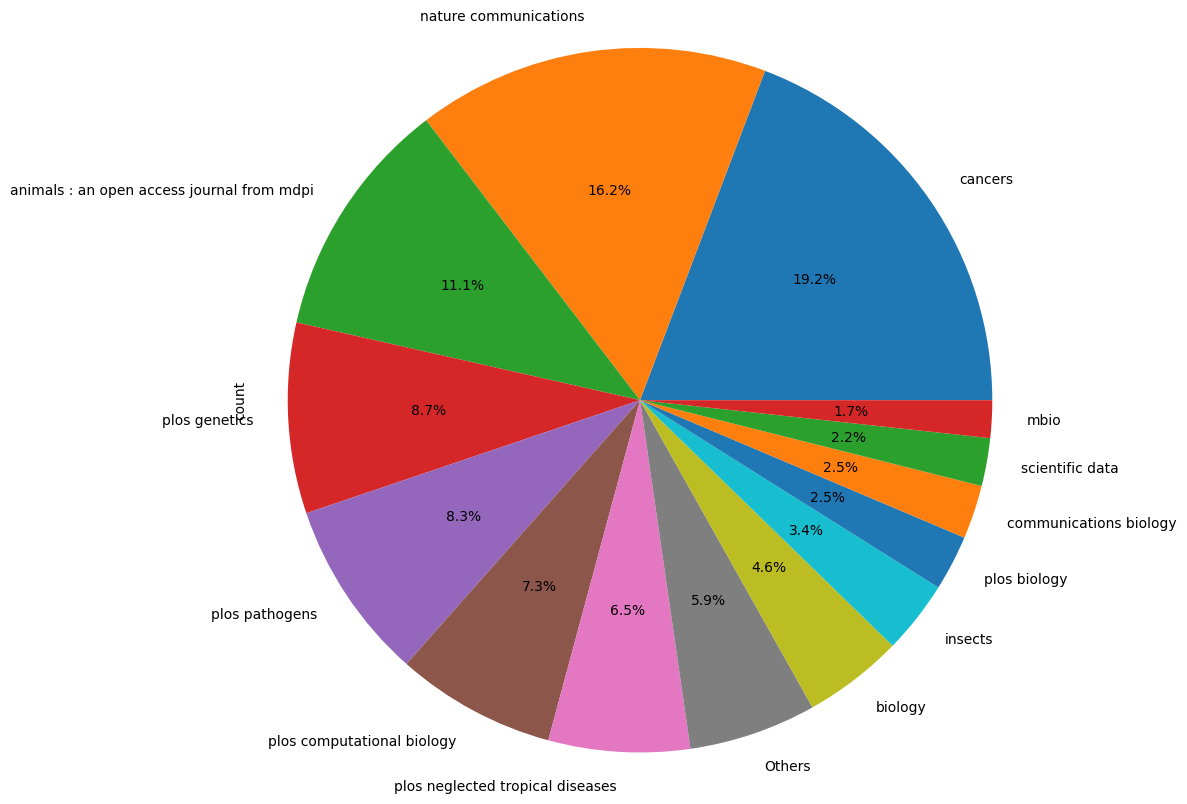
\includegraphics[width=\textwidth]{images/journal_instances_percentage.png}
    \caption{Distribuzione percentuale delle istanze per rivista.}
    \label{fig:journal-inst-perc}
\end{figure}


La suddivisione ha seguito fedelmente la distribuzione mostrata nella figura in questione, cioè si sono generati 13 subset oltre a quello che comprende le riviste con meno istanze. 
La tabella \ref{tab:split-journals} mostra in termini numerici la dimensione di ogni subset.

\begin{table}
\centering
\begin{tabular}{|l|c|c|c|}
\hline
       & train & validation & test \\
\hline
all    & 35026 & 4380       & 4384 \\
NC     & 5549  & 694        & 694  \\
A      & 3909  & 489        & 489  \\
PLGEN  & 3087  & 386        & 386  \\
PLPAT  & 2920  & 365        & 365  \\
PLCB   & 2589  & 324        & 324  \\
PLNTD  & 2289  & 286        & 287  \\
B      & 1617  & 202        & 203  \\
I      & 1181  & 148        & 148  \\
PLB    & 896   & 112        & 113  \\
CB     & 867   & 108        & 109  \\
SD     & 725   & 91         & 91   \\
MBIO   & 607   & 76         & 76   \\
C      & 6782  & 848        & 848  \\
OTHER  & 2008  & 251        & 251  \\
\hline
\end{tabular}
\caption{Dimensione numerica di ogni subset.}
\label{tab:split-journals}
\end{table}

Per questioni di sintesi, i nomi delle riviste sono stati abbreviati come segue:
\begin{itemize}
    \item NC: Nature Communications.
    \item A: Animals : An Open Access Journal from MDPI.
    \item PLGEN, PLAPAT, PLCB, PLNTD, PLB: PLoS \{Genetics, Pathogens, Computational Biology, Neglected Tropical Diseases, Biology\}.
    \item B: Biology.
    \item I: Insects.
    \item CB: Communications Biology.
    \item SD: Scientific Data.
    \item MBIO: mBio.
    \item C: Cancers.
\end{itemize}


\section{Upload del dataset su HuggingFace}
Come ultima operazione effettuata sui dati, si è deciso di caricare l'intero dataset su \href{https://huggingface.co/}{\emph{HuggingFace}} nel repository intitolato, per l'appunto, \href{https://huggingface.co/datasets/paniniDot/sci_lay}{\emph{sci\_lay}}. 
Hugging Face è diventata una delle principali piattaforme per il Natural Language Processing (NLP) e il Deep Learning, offrendo un'ecosistema completo per la formazione, il testing e la distribuzione di modelli di linguaggio. Caricare un dataset su Hugging Face può offrire una serie di vantaggi chiave, in particolare per la comunità di ricercatori e sviluppatori. Ecco una descrizione dei motivi principali:

\begin{itemize}
    \item \textbf{Accessibilità}: Una volta caricato su Hugging Face, il dataset diventa facilmente accessibile a chiunque nella comunità. Questo permette ad altri ricercatori e sviluppatori di sfruttare il dataset senza passare attraverso processi di download e setup complicati.
    \item \textbf{Standardizzazione}: Hugging Face offre una struttura standardizzata per i dataset, rendendo più semplice per gli utenti navigare, comprendere e utilizzare diversi dataset in modo coerente. 
    \item \textbf{Integrazione con Modelli}: Hugging Face non è solo una piattaforma per dataset, ma anche per modelli di linguaggio. Caricando un dataset lì, si facilita la formazione, il fine-tuning e la valutazione dei modelli usando quella specifica risorsa, tutto all'interno dello stesso ecosistema.
    \item \textbf{Versioning}: Proprio come per i software, i dataset possono subire modifiche e revisioni nel tempo. Hugging Face supporta il versioning, permettendo agli utenti di accedere a diverse versioni del dataset e tracciare le modifiche. Nel caso di SciLay, ad esempio, il dataset è disponibile solo nella versione $1.0.0$ (cased) che dispone degli articoli con caratteri maiuscoli e minuscoli.
    \item \textbf{Documentazione e Metadati}: La piattaforma permette di fornire documentazione dettagliata, basata sul concetto di \emph{Dataset Card} proposta nell'articolo ``Data Cards: Purposeful and Transparent Dataset Documentation for Responsible AI''\cite{pushkarna2022data}, e metadati associati al dataset. In questo modo si aiutano gli utenti a comprendere e utilizzare al meglio la risorsa.
\end{itemize}

In conclusione, caricare un dataset su Hugging Face non solo semplifica la distribuzione e l'adozione della risorsa, ma promuove anche la standardizzazione, la collaborazione e l'innovazione nell'ambito del Natural Language Processing e delle discipline correlate. 


%% CAPITOLO 2
\chapter{Le tecnologie disponibili}
\label{cap:ml}

Nella successiva sezione, viene presentata una descrizione dettagliata degli strumenti utilizzati per realizzare gli obiettivi di questo progetto. Dopo un breve inquadramento del \emph{Machine Learning}, ci concentreremo sul \emph{Natural Language Processing}, dando particolare enfasi alle metodologie contemporanee più avanzate per la comprensione, generazione e sintesi del testo.

\section{Machine Learning}
Il Machine Learning, spesso abbreviato come ML, è un sottoinsieme dell'intelligenza artificiale che riguarda l'uso di algoritmi e modelli statistici per consentire ai computer di eseguire un compito senza l'uso di istruzioni esplicite. Invece, si basa su modelli che apprendono e si adattano alle informazioni e ai dati di input per prendere decisioni o effettuare previsioni senza essere esplicitamente programmati per farlo.
Uno dei riferimenti più autorevoli in materia è Tom Mitchell, che ha fornito una definizione ben accettata di apprendimento automatico\cite{DBLP:books/daglib/0087929}:

\begin{quote}
    \emph{
    Si dice che un programma apprende dall'esperienza $E$ con riferimento ad alcune classi di compiti $T$ e con misurazione della performance $P$, se le sue performance nel compito $T$, come misurato da $P$, migliorano con l'esperienza $E$.}
\end{quote}

Questa definizione sottolinea l'idea centrale che, nel Machine Learning, un algoritmo migliora la sua performance nel tempo attraverso l'esperienza, che è tipicamente fornita sotto forma di dati di addestramento.
Questo processo emula il \emph{ragionamento induttivo} umano, essenziale per identificare tendenze o schemi, dando origine al concetto di \emph{pattern recognition}. A differenza degli algoritmi classici, questi sistemi operano in modo probabilistico, implicando che le relazioni identificate potrebbero non essere universalmente valide, ma piuttosto influenzate dai dati iniziali. La modalità di induzione più diffusa è la \emph{generalizzazione}, che permette di dedurre informazioni riguardanti un intero insieme basandosi sull'analisi di una sua parte.
Nello specifico i modelli di Machine Learning si basano proprio sul concetto di generalizzazione per portare a compito task, anche estremamente complicati da codificare esplicitamente. 

\subsection{La scelta dei dati}
Quanto appena detto fa comprendere come il ruolo dei dati sia cruciale in questo tipo di sistemi. Maggiore è la quantità di dati e più tendenzialmente il modello sarà in grado di generalizzare correttamente e dunque fare previsioni corrette sottoponendo nuove istanze rispetto a quelle su cui si è addestrato. 
Questo concetto evidenzia anche la rinascita del Machine Learning degli ultimi due decenni. Col tempo, si è riconosciuta l'importanza vitale dei dati nella costruzione di modelli efficaci per supportare decisioni o effettuare previsioni in ambiti applicativi complessi. Di conseguenza, c'è stata una tendenza crescente alla raccolta e conservazione di grandi quantità di dati. Parallelamente, grazie all'avanzamento dell'hardware, che ha seguito la legge di Moore (anche se recentemente si sono manifestati segnali di un possibile rallentamento a causa delle limitazioni fisiche dei transistor), la capacità di elaborazione dei dati è cresciuta esponenzialmente. Questo ha reso possibile l'addestramento di modelli di Machine Learning sempre più sofisticati.
Un aspetto da non sottovalutare è che quantità non coincide sempre con qualità. In altre parole, seguendo il principio ``\emph{Garbage In, Garbage Out}'' (GIGO), dati inesatti, incompleti o distorti possono portare a risultati errati o fuorvianti, nonché a decisioni ingiuste o discriminatorie.
Risulta pertanto cruciale prestare attenzione alla rappresentatività e all'equità durante la raccolta e la preparazione dei dati.
Un noto esempio inerente è il caso \emph{COMPAS}, riguardante un algoritmo utilizzato negli Stati Uniti per valutare il rischio di recidiva dei criminali. Esso ha sollevato molte preoccupazioni in merito alle questioni di equità e bias, soprattutto dopo che un'inchiesta da parte di ProPubblica che prese il nome di ``\emph{Machine Bias}''\cite{compas} ha suggerito che l'algoritmo potrebbe essere sbilanciato contro i detenuti afroamericani.
In sintesi, i dati sono la colonna vertebrale del Machine Learning. La selezione, la preparazione e l'uso corretto dei dati determinano in gran parte il successo di qualsiasi progetto di ML. Una gestione attenta e riflessiva dei dati può fare la differenza tra un modello efficace e uno inefficace.


\subsection{Perché Machine Learning?}
Il machine learning rappresenta oggi uno dei pilastri fondamentali nell'ambito dell'intelligenza artificiale. Giganti tecnologici come Google, Microsoft e Netflix investono considerevoli risorse finanziarie nella ricerca di soluzioni innovative che possano elevare la qualità dell'esperienza degli utenti, traducendosi in un aumento dei loro profitti. La ricerca nel campo è in costante evoluzione, con la comunità scientifica che offre contributi preziosi in diversi settori:
\begin{itemize}
    \item \textbf{Riconoscimento delle immagini}. 
    Il ML, in particolare le reti neurali convoluzionali (CNN), ha rivoluzionato il riconoscimento e la classificazione delle immagini. Servizi come Google Photos e piattaforme di social media utilizzano il ML per riconoscere oggetti, volti e scene nelle immagini.
    \item \textbf{Elaborazione del linguaggio naturale (NLP)}. Il ML ha portato a progressi significativi nel riconoscimento vocale, nella traduzione automatica, nella generazione di testo e nell'analisi del sentimento. Siri di Apple, Google Translate e GPT-3 (e 4) di OpenAI sono esempi di applicazioni NLP basate su ML.
    \item \textbf{Raccomandazioni personalizzate}. Piattaforme come Netflix, Spotify e Amazon utilizzano algoritmi di ML per fornire raccomandazioni personalizzate agli utenti in base alle loro preferenze e comportamenti passati.
    \item \textbf{Veicoli autonomi}. Il ML è essenziale per le funzioni di guida autonoma, come il riconoscimento di ostacoli, la previsione del comportamento di altri utenti della strada e la decisione sul percorso da seguire.
\end{itemize}

Il vero valore aggiunto del machine learning, come già detto, risiede nella sua capacità di apprendimento e generalizzazione. L'incremento delle performance è spesso correlato alla quantità di dati disponibili, rendendo questi sistemi particolarmente adatti a gestire situazioni reali di elevata complessità, spesso al di là della capacità dei tradizionali algoritmi deterministici. La natura autoapprendente di queste tecniche permette di semplificare lo sviluppo di applicazioni, poiché l'algoritmo stesso si adatta autonomamente al contesto in cui opera.




\subsection{Sviluppo di un modello}

Come anticipato, ogni algoritmo di Machine Learning ha l'obiettivo di "imparare" dalle relazioni presenti nei dati forniti, in modo da poter "generalizzare", ovvero effettuare previsioni accurate su nuovi dati mai visti prima.
Occorre dunque definire matematicamente cosa significa trovare delle relazioni fra i dati. Formalmente siano $\mathbf{x} \in \mathbb{R}^n$ (con $n \geq 1$) un vettore di dati di input e un output $y \in \mathbb{R}$. Se vale
\begin{equation}\label{eq:rel_modello}
    y = h(\mathbf{x}) = \theta_1 x_1 + \theta_2 x_2 + \cdots + \theta_n x_n + \beta
\end{equation}
possiamo affermare che esiste una qualche relazione tra $\mathbf{x}$ e $y$.
La funzione $h$ che lega le premesse ($\mathbf{x}$) alla conclusione ($y$) rappresenta un \emph{modello}, e i coefficenti $\theta_i$ i suoi parametri. 
In sostanza, un modello è una rappresentazione matematica di un fenomeno, che cerca di descrivere le relazioni tra le variabili basandosi su osservazioni passate.

L'obiettivo principale nel Machine Learning è trovare un modello $h$ che rappresenti al meglio le relazioni nel dominio di interesse. Formalmente, dunque, se l'equazione \ref{eq:rel_modello} lega input e output di una specifica istanza, qualora disponessimo di $m \geq 1$ istanze d'esempio, vorremmo determinare una funzione che riduca al minimo la discrepanza tra ogni output reale e l'output previsto dal modello. Questa quantità è definita \emph{errore del modello}.
Dato l'esempio $i-$esimo, siano $y_i$ l'output reale e $y_i'$ l'output previsto, allora trovare il modello migliore significa ottenere i parametri $\theta_i$ tali che si minimizzi l'errore di previsione.
Poiché l'errore è funzione dei parametri, lo denoteremo come $E(\mathbf{\theta})$ dove $\mathbf{\theta}$ è il vettore dei parametri. Allora avremo

\begin{align*}
    E(\mathbf{\theta}) &=\text{min } \sum_{i=1}^m \frac{1}{2}(y_i - y_i')^2 \\
    &=\text{min } \sum_{i=1}^m \frac{1}{2}\left(y_i - h\left(\mathbf{x}_i\right)\right)^2
\end{align*}

L'errore è rappresentato utilizzando la media dei quadrati degli errori (anche detto \emph{errore quadratico medio} RMSE) per questioni di trattabilità matematica. La funzione in questione è differenziabile e pertanto è possibile l'uso di tecniche di ottimizzazione come la \emph{discesa del gradiente} che tratteremo nella sezione successiva.

\paragraph{Esempio}
Quando abbiamo $n=1$, ci troviamo in un contesto bidimensionale, con una dimensione dedicata alla variabile indipendente e l'altra alla variabile dipendente. Con $m \geq 1$ osservazioni disponibili, possiamo visualizzare il nostro modello $h$ su un grafico cartesiano. Se le previsioni del modello si allineano lungo una retta, ci riferiamo a questo come \emph{regressione lineare}. Il grafico potrebbe apparire come:

\begin{figure}[H]
    \centering
    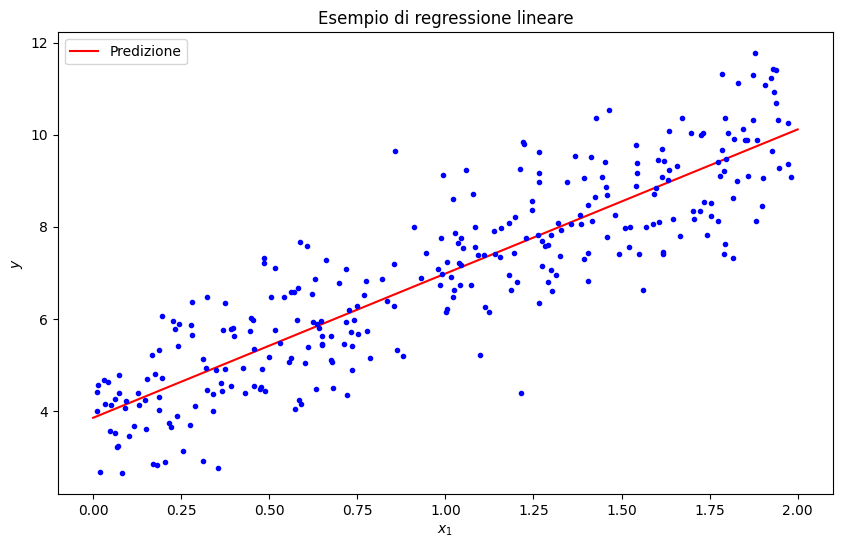
\includegraphics[width=\textwidth]{images/regr_lin.png}
    \caption{Esempio di regressione lineare.}
    \label{fig:lin-reg}
\end{figure}

Dove la retta $y = \theta x$ è stata calcolata in modo che il valore di $\theta$ minimizzi la somma dell'errore quadratico medio rispetto a tutti i punti $(x_i, y_i)$ d'esempio. 


\subsection{Ricerca dei parametri: discesa del gradiente}
\label{gradiente}

Fino a questo momento abbiamo parlato di auto apprendimento della macchina in maniera del tutto generale, lasciando spazio alle ipotesi più fantasiose, fra cui l'idea che la macchina abbia un'effettiva intelligenza, simile a quella umana. In realtà, il modo in cui i sistemi auto apprendono è semplicemente quello di ricercare i parametri migliori (secondo quanto detto prima) per un determinato dominio applicativo. Ma come si trovano questi parametri? 
L'approccio più generale è chiamato \emph{discesa del gradiente} che non è altro che un algoritmo di ottimizzazione utilizzato per minimizzare una funzione obiettivo attraverso aggiornamenti iterativi. Nel nostro caso la funzione obbiettivo da minimizzare sarà ovviamente $E(\mathbf{\theta})$, cioè l'errore quadratico medio sulla predizione.
Essendo $E(\mathbf{\theta})$ una funzione, l'interpretazione geometrica di questo processo è di percorrere la curva lungo il punto in cui ha pendenza maggiore fino a trovare un minimo locale (o globale che sia).
Il vettore direzione che ci indica verso dove avanzare alle iterazioni successive è chiamato, appunto, \emph{gradiente}.
Dal punto di vista matematico, poiché l'errore è funzione di $\theta$, ovvero il vettore dei parametri dati alle variabili indipendenti, ci troveremo in uno spazio di $n+1$ dimensioni, dove $n$ corrisponde al numero di parametri. Supponendo di avere $n=2$ parametri graficamente avremo

\begin{figure}[H]
    \centering
    \begin{subfigure}[b]{0.48\textwidth}
        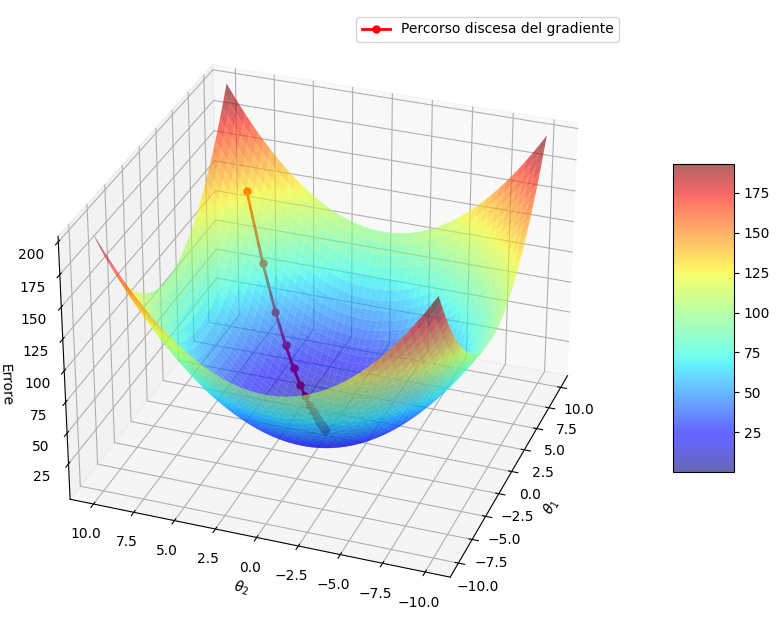
\includegraphics[width=\textwidth]{images/gradiente.png}
    \end{subfigure}
\quad
    \begin{subfigure}[b]{0.48\textwidth}
        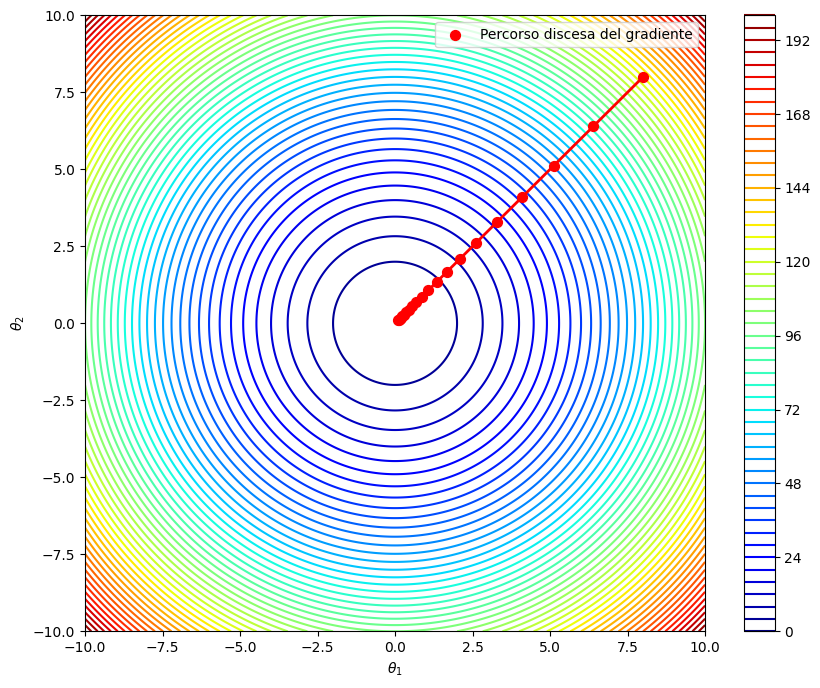
\includegraphics[width=\textwidth]{images/gradiente2.png}
    \end{subfigure}
    \caption{Rappresentazione grafica discesa del gradiente per un modello a due parametri.}
    \label{fig:grad-descent}
\end{figure}


Formalmente, il gradiente corrisponde al vettore delle derivate parziali della funzione errore rispetto a ogni parametro. Se si ha un solo parametro, il gradiente si identifica con la derivata della funzione errore. Dal punto di vista matematico le derivate forniscono la pendenza istantanea di una curva in un qualsiasi punto essa sia calcolata (ammesso che sia sempre derivabile, cosa vera per $E(\theta)$ essendo MSE). Perciò, muovendosi nella direzione opposta al gradiente, si procede nella maniera più efficiente possibile, poiché in tale direzione la funzione decresce al tasso più veloce.

Considerando $E(\theta)$ come la funzione da minimizzare, il suo gradiente si calcola come
\begin{align*}
    \nabla E(\theta) = \begin{bmatrix}
        \frac{\partial E}{\partial \theta_1} \\
        \frac{\partial E}{\partial \theta_2} \\
        \vdots \\
        \frac{\partial E}{\partial \theta_n}
    \end{bmatrix}
\end{align*}

A questo punto, per minimizzare $E$, aggiorniamo iterativamente il vettore dei parametri $\theta$ nella direzione opposta al gradiente. Definiamo come $\theta$ il vettore dei parametri all'iterazione precedente e $\theta'$ quello all'iterazione corrente. L'aggiornamento è dato da 
\begin{equation}\label{eq:discesa_gradiente}
    \theta' = \theta - \alpha \nabla E(\theta)
\end{equation}
dove $\alpha$ è un cosiddetto \emph{iperparametro}, ovvero un parametro con cui regolare le modalità in cui il modello apprende. Questo determina l'ampiezza da percorrere ad ogni iterazione. Un $\alpha$ troppo grande potrebbe far ``saltare'' il minimo, mentre uno troppo piccolo potrebbe rendere la convergenza troppo lenta.

Il processo si ripete fino al soddisfacimento di un \emph{criterio d'arresto}. Tale criterio può basarsi su diversi fattori:

\begin{itemize}
\item Arresto quando l'errore scende sotto una soglia predeterminata.
\item Arresto dopo un numero predefinito di iterazioni.
\end{itemize}


\subsection{Validazione del modello}
Per capire se il modello è effettivamente valido (da qui il nome \emph{validazione}) a descrivere un certo dominio applicativo si possono utilizzare due differenti approcci.
\begin{enumerate}
    \item Il metodo \emph{hold-out} rappresenta una delle strategie più elementari e diffuse per determinare l'efficacia di un modello di apprendimento automatico. Consiste essenzialmente nella suddivisione dell'insieme di dati in due segmenti distinti: uno dedicato all'addestramento del modello e l'altro alla sua validazione. Queste due porzioni sono frequentemente denominate \emph{train} e \emph{test} set.
    È usuale destinare tra il 70-80\% dell'insieme dei dati all'addestramento e il rimanente 20-30\% alla validazione, anche se tali percentuali possono essere adattate in base al contesto e alla mole di dati a disposizione.
    Il set di addestramento è impiegato per istruire il modello. Al termine di tale fase, il modello è sottoposto a verifica utilizzando il set di test. Poiché questi dati non sono stati utilizzati durante la fase di addestramento, consentono di valutare le capacità del modello nell'affrontare dati inediti.
    È inoltre praticabile una segmentazione ulteriore dell'insieme dei dati, introducendo un \emph{set di validazione}. Quest'ultimo è utilizzato per rifinire gli iperparametri del modello, mirando al miglioramento delle sue prestazioni. Conclusa questa ottimizzazione, il modello è nuovamente addestrato e, successivamente, la sua efficacia è testata con il set di test.
    È tuttavia essenziale considerare che l'affidabilità della valutazione potrebbe oscillare in base alla modalità di divisione dei dati. Se il set di test non risulta rappresentativo dell'intero insieme di dati, si potrebbero registrare incoerenze nella valutazione.
    \item La soluzione ai limiti dell'hold out arriva dalla \emph{$k-$fold cross validation} la quale mira a ottenere una valutazione più robusta e meno sensibile alle fluttuazioni che potrebbero derivare da una singola suddivisione casuale dei dati in set di addestramento e test, come avviene nel metodo hold-out. L'intero set di dati viene suddiviso in $k$ sottoinsiemi (o ``fold'') di dimensioni approssimativamente uguali. La procedura di addestramento e test viene ripetuta $k$ volte. Ogni volta, uno dei $k$ fold viene utilizzato come set di test, mentre gli altri $k-1$ fold vengono combinati per formare il set di addestramento. Pertanto, ogni dato nel set viene utilizzato esattamente una volta come dato di test. In questo modo l'errore finale è dato dalla somma degli errori di previsione sui singoli test. Questo fa si che l'errore trovato sia più generale e meno influenzato dai dati scegli per addestrarlo.
\end{enumerate}

Qualora a seguito della validazione del modello ci si rende conto che il modello non è in grado di generalizzare adeguatamente bene su nuovi dati non visti durante la fase di addestramento, possono presentarsi due problematiche.
\begin{enumerate}
    \item \emph{Underfitting}. Si verifica quando un modello è troppo semplice per catturare la struttura sottostante dei dati. Di conseguenza, il modello potrebbe avere una cattiva performance sia sul set di addestramento che sul set di test. Le ragioni per cui questo accade possono essere svariate, ma le più frequenti sono la scelta di un modello troppo semplice per descrivere le relazioni fra dati, la presenza di troppi pochi parametri o ancora l'addestramento effettuato per troppe poche iterazioni.
    \item \emph{Overfitting}. Si verifica quando un modello è troppo complesso e inizia a ``imparare'' anche il rumore presente nei dati di addestramento, anziché la struttura sottostante dei dati stessi. In pratica, un modello che soffre di overfitting avrà ottime prestazioni sul set di addestramento, ma avrà prestazioni scarse sul set di test o su nuovi dati non visti.
\end{enumerate}

Questo ci permette di capire che nel ML, di essenziale importanza è bilanciare la complessità del modello con la quantità e la qualità dei dati a disposizione, e monitorare attentamente le prestazioni del modello sia sul set di addestramento che sul set di test.


\begin{figure}[H]
\centering
    \begin{subfigure}[b]{0.3\textwidth}
    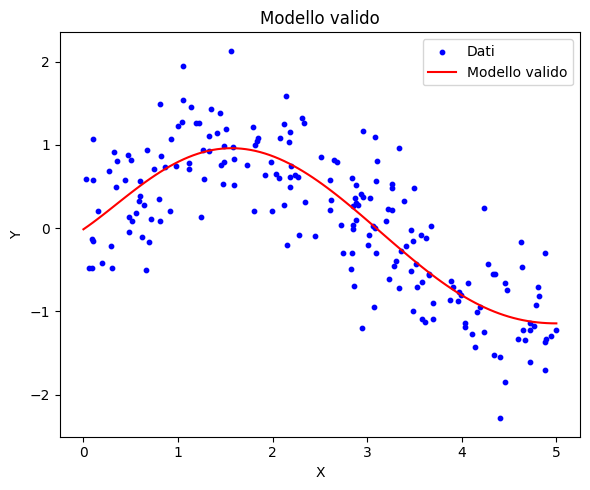
\includegraphics[width=\textwidth]{images/valido.png}
    \caption{Modello rappresentativo dei dati.}
    \end{subfigure}
\quad
    \begin{subfigure}[b]{0.3\textwidth}
    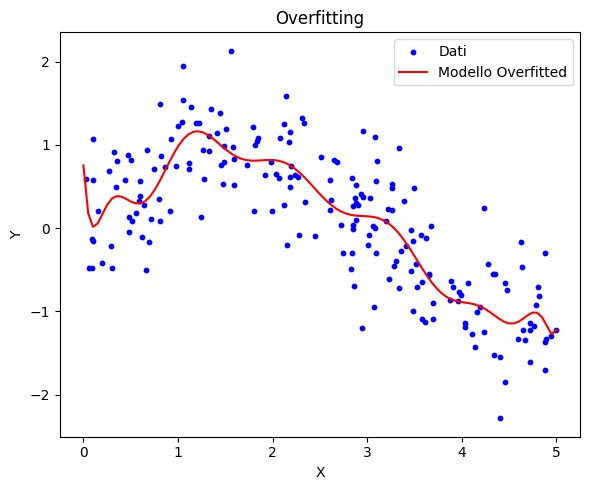
\includegraphics[width=\textwidth]{images/overfitting.png}
    \caption{Modello affetto da overfitting.}
    \end{subfigure}
\quad
    \begin{subfigure}[b]{0.3\textwidth}
    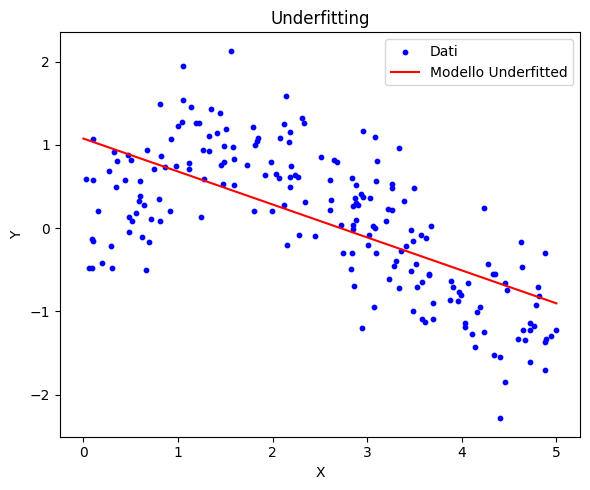
\includegraphics[width=\textwidth]{images/underfitting.png}
    \caption{Modello affetto da underfitting.}
    \end{subfigure}
\caption{}
\label{fig:over_under_fitting}
\end{figure}


\section{Reti Neurali}
Le \emph{reti neurali} rappresentano un pilastro centrale nel campo del machine learning. Sono modelli computazionali che traggono ispirazione dalla struttura e dalle funzionalità del cervello umano, progettati per replicare il modo in cui gli esseri umani apprendono e processano le informazioni. Il parallelo con il cervello umano, seppure non stretto, serve come modello concettuale per comprendere i principi di base del loro funzionamento.

\subsection{Struttura e Componenti di una Rete Neurale}
Le reti neurali sono formate da unità di calcolo denominate, appunto, \emph{neuroni} o \emph{nodi}, raggruppate in strati, o \emph{layers}. Questi si dividono in tre categorie principali:
\begin{itemize}
    \item \emph{Input layer}: rappresenta il punto di ingresso della rete, dove sono ricevuti gli input esterni.
    \item \emph{Hidden layers} (strati nascosti): possono essere plurimi e, più sono numerosi, più la rete è in grado di gestire complessità, migliorando le proprie performance. Qui, i dati in ingresso sono elaborati ulteriormente.
    \item \emph{Output layer}: è l'ultimo strato, attraverso il quale la rete fornisce i risultati dell'elaborazione dei dati in input.
\end{itemize}

\subsubsection{Funzionamento di un Neurone}
La figura \ref{fig:neurone} illustra schematicamente il funzionamento di una singola unità neuronale. Ogni neurone riceve in input gli output di $n$ neuroni connessi a esso. Ogni connessione $i$ ha associato un \emph{peso} $w_i$, ottimizzato durante la fase di addestramento del modello. Il neurone moltiplica ogni input $x_i$ per il peso corrispondente, somma i prodotti ottenuti e aggiunge un \emph{bias} $b$ determinato anch'esso in fase di addestramento. Questa quantità è detta \emph{somma ponderata degli input}.
Questo bias è necessario per consentire al neurone di avere un grado di libertà aggiuntivo nel processo di apprendimento. Maggiore libertà comporta una maggiore adattabilità ai dati di addestramento.
Questa operazione produce la \emph{somma ponderata degli input}. Il bias fornisce al neurone un grado di libertà supplementare, permettendogli di adattarsi meglio ai dati durante la fase di apprendimento. La somma ponderata è poi processata da una \emph{funzione di attivazione} che decide se il neurone deve essere attivato o meno, introducendo una componente di \emph{non-linearità} essenziale per l'apprendimento di rappresentazioni complesse e relazioni non-lineari tra input e output. La formula appena descritta è la seguente:
\begin{equation*}
    \hat{y} = g(\mathbf{w \cdot x} + b) = g\left( \sum_{i=1}^n w_i \cdot x_i + b \right) 
\end{equation*}

\begin{figure}[H]
    \centering
    \begin{tikzpicture}
        % Neuron
        \node[draw, circle, minimum size=1.5cm] (sum) at (0,0) {$\Sigma$};
        
        % Inputs
        \def\numInputs{4}
        \foreach \i in {1,2,...,\numInputs} {
            \ifnum\i=3
                \node at (-3, \numInputs - \i*1.5) {$\vdots$};
            \else
                \ifnum\i=4
                    \node[draw, circle, minimum size=0.5cm] (input\i) at (-3, \numInputs - \i*1.5) {$x_n$};
                    \draw[->] (input\i) -- (sum) node[midway, above] {$w_n$};
                \else
                    \node[draw, circle, minimum size=0.5cm] (input\i) at (-3, \numInputs - \i*1.5) {$x_\i$};
                    \draw[->] (input\i) -- (sum) node[midway, above] {$w_\i$};
                \fi
            \fi
        }
    
        % Bias
        \node[minimum size=0.5cm] (bias) at (0, 2.5) {$b$};
        \draw[->] (bias) -- (sum);
    
        % Activation
        \node[draw, circle, minimum size=1.5cm] (act) at (3, 0) {$g(\cdot)$};
        \draw[->] (sum) -- (act);
    
        % Output
        \node[minimum size=0.5cm] (output) at (6, 0) {$\hat{y}$};
        \draw[->] (act) -- (output);    
    
    \end{tikzpicture}
    \caption{Schema di funzionamento unità neuronale.}
    \label{fig:neurone}
\end{figure}

\subsubsection{Funzioni di Attivazione}
Le funzioni di attivazione si classificano principalmente in due categorie, in base al loro codominio: 
\begin{itemize}
    \item \emph{Funzioni di attivazione normalizzate}: queste funzioni, ad esempio, mappano i reali in intervalli del tipo $[0,1]$ o $[-1, 1]$, risultando particolarmente utili nei layer di output quando la rete deve produrre probabilità, come nei task di classificazione. Alcuni esempi includono:
    \begin{itemize}
        \item \emph{Sigmoide}. Può essere utile nella classificazione binaria poiché è definita in $\mathbb{R} \rightarrow [0,1]$. Si ottiene con
        \begin{equation*}
            \sigma(x) = \frac{1}{1+e^{-x}}
        \end{equation*}
        \item \emph{Tangente iperbolica}. Definita in $\mathbb{R} \rightarrow [-1,1]$ e vale
        \begin{equation*}
            \tanh(x) = \frac{2}{1+e^{-2x}} - 1
        \end{equation*}
    \end{itemize}
    \item \emph{Funzioni di attivazione continue}: queste mappano  $\mathbb{R} \rightarrow \mathbb{R}$. e l'output determina non solo se il neurone è attivato, ma anche la quantità di segnale trasmesso. Un esempio noto è la \emph{ReLU} (Rectified Linear Unit) ed è definita in $\mathbb{R} \rightarrow \mathbb{R}^+$. Se si attiva trasmette un segnale proporzionale alla somma pesata degli input, infatti è definita come
    \begin{equation*}
        \text{ReLU}(x) = \text{max}(0, x)
    \end{equation*}
    Se l'input ($x$) è negativo, il neurone restituisce 0, interpretato come uno ``spegnimento'' del neurone; se positivo, il neurone restituisce l'input ricevuto.
\end{itemize}

\subsection{Processo di Addestramento}
Durante l'addestramento di una rete neurale, come precedentemente menzionato, si scelgono i pesi delle connessioni tra neuroni e i bias di questi, in modo da rappresentare al meglio i dati di esempio. Analogamente agli algoritmi di Machine Learning (ML) tradizionali, l'accuratezza del modello viene valutata mediante una funzione d'errore, nota come \emph{loss function}, che quantifica la divergenza del modello dalla soluzione desiderata. Il valore ottenuto, frequentemente denominato perdita'' o errore'', è indicativo dell'accuratezza del modello: valori bassi sono indice di predizioni precise, mentre valori alti denotano predizioni inesatte. L'obiettivo durante la fase di addestramento è minimizzare il valore della funzione di perdita.
Per ridurre la loss, si adotta l'approccio della discesa del gradiente (vedi paragrafo \ref{gradiente}). In particolare, ad ogni iterazione, comunemente definita come \emph{``epoca di addestramento''} nel contesto delle reti neurali, si procede attraverso i seguenti passaggi:
\begin{itemize}
\item Si effettuano predizioni sui dati di esempio basandosi sui parametri attuali del modello.
\item Si calcola la loss confrontando le predizioni con i valori reali.
\item Si determina il gradiente della funzione di perdita rispetto ai parametri attuali del modello.
\item Si aggiornano i parametri del modello muovendosi nella direzione che minimizza la funzione di perdita, come descritto dall'equazione \ref{eq:discesa_gradiente}.
\end{itemize}

\subsection{Reti Neurali Feed-forward (FNN)}
Le reti neurali di tipo \emph{feedforward}, quali ad esempio i Multilayer Perceptron, rappresentano le forme più elementari e fondamentali di reti neurali. Questi modelli sono caratterizzati da un flusso d’informazione che procede in un’unica direzione, andando dal layer di input, passando per gli eventuali layer nascosti, fino a raggiungere il layer di output. In queste strutture, il processo attraverso il quale l’informazione è inviata da un neurone all’altro è conosciuto come \emph{forwarding}.
Nel dettaglio, in un'architettura feedforward, ogni neurone è interconnesso con tutti i neuroni presenti nel layer immediatamente successivo, formando una rete densamente connessa in cui l'informazione si muove in modo ordinato e strutturato da uno strato all'altro, senza cicli o ritorni. Questa struttura rigidamente organizzata si contrappone a modelli più complessi, come le reti \emph{neurali ricorrenti} (trattate nel paragrafo successivo), che permettono connessioni in entrata anche da neuroni situati nello stesso layer o in layer successivi.
Analizzando più profondamente il funzionamento di ogni singolo neurone, come illustrato nella figura \ref{fig:neurone}, è possibile notare che tutti gli input ricevuti da un neurone provengono esclusivamente da neuroni situati nel layer precedente, e ogni output prodotto è destinato unicamente ai neuroni del layer successivo. Ciò implica che ogni neurone opera come una sorta di stazione di transito, ricevendo segnali in ingresso, elaborandoli e inoltrandoli ai neuroni successivi, contribuendo così alla progressiva trasformazione dell'input iniziale fino all'ottenimento dell'output finale.
Nelle reti neurali feedforward, i layer nascosti hanno il compito di elaborare e trasformare progressivamente le informazioni in ingresso, estraendo e combinando caratteristiche e rappresentazioni ad alto livello, indispensabili per l'esecuzione di compiti complessi. La presenza di più layer nascosti, ciascuno con un numero variabile di neuroni, consente alla rete di modellare relazioni e pattern sempre più complessi e astratti, aumentando la sua capacità di apprendimento e generalizzazione.
La figura \ref{fig:fnn} mostra un esempio di rete neurale feedforward, composta da un layer di input, tre layer nascosti e un layer di output. In questa rappresentazione grafica, è possibile osservare la strutturazione gerarchica e sequenziale della rete e l'organizzazione delle connessioni tra i diversi neuroni, che evidenzia la natura unidirezionale e strutturata del flusso informativo all'interno del modello.


\begin{figure}[H]
    \centering
    \begin{tikzpicture}[>=stealth, neuron/.style={circle, draw, minimum size=0.5cm}, font=\footnotesize]

        % Neuroni
        \foreach \i in {1,...,7} \node[neuron] (I-\i) at (0,\i) {};
        \foreach \i in {1,...,5} \node[neuron] (H1-\i) at (2.5,\i + 1) {};
        \foreach \i in {1,...,3} \node[neuron] (H2-\i) at (5,\i + 2) {}; 
        \foreach \i in {1,...,5} \node[neuron] (H3-\i) at (7.5,\i + 1) {};
        \foreach \i in {1,...,3} \node[neuron] (O-\i) at (10,\i + 2) {}; 
        
        % Connetti neuroni
        \foreach \i in {1,...,7} \foreach \j in {1,...,5} \draw[->] (I-\i) -- (H1-\j);
        \foreach \i in {1,...,5} \foreach \j in {1,...,3} \draw[->] (H1-\i) -- (H2-\j);
        \foreach \i in {1,...,3} \foreach \j in {1,...,5} \draw[->] (H2-\i) -- (H3-\j);
        \foreach \i in {1,...,5} \foreach \j in {1,...,3} \draw[->] (H3-\i) -- (O-\j);
        
        % Nodi titoli dei layer
        \node[below=of I-4, yshift=-2cm] (IL) {Input Layer}; 
        \node[below=of H1-3, yshift=-2cm] (H1L) {Hidden Layer 1};
        \node[below=of H2-2, yshift=-2cm] (H2L) {Hidden Layer 2};
        \node[below=of H3-3, yshift=-2cm] (H3L) {Hidden Layer 3};
        \node[below=of O-2, yshift=-2cm] (OL) {Output Layer};
    
    \end{tikzpicture}
    \caption{Feedforward Neural Network.}
    \label{fig:fnn}
\end{figure}



\subsection{Reti Neurali Ricorrenti (RNN)}
Le \emph{reti neurali ricorrenti} (RNN) sono una classe speciale di reti neurali che sono particolarmente efficaci nel trattare sequenze di dati, come serie temporali o sequenze di testo. A differenza delle reti neurali feedforward (FNN), le RNN sono in grado di mantenere uno stato interno che cattura le informazioni relative alle parti precedenti della sequenza.
In particolare le FNN presentano limitazioni significative quando si tratta di elaborare dati sequenziali o temporali (si pensi ad esempio a tutti quei task che coinvolgono testo dove per comprendere una frase è necessario avere contezza del significato delle parole precedenti in relazione a quella attuale). In particolare
\begin{itemize}
    \item \emph{Mancanza di memoria temporale}. Le FNN non hanno memoria interna o stato che può catturare l'ordine o la sequenza delle informazioni, rendendole inefficienti per problemi che richiedono la considerazione del contesto temporale o sequenziale. Le informazioni fluiscono senza lasciare traccia all'interno della rete. Ogni input è considerato a se stante. 
    \item \emph{Dimensione fissa dell'input}. Le FNN richiedono che l'input sia di dimensione fissa, il che è limitante per l'elaborazione di sequenze di lunghezza variabile. Infatti, come mostra figura \ref{fig:fnn}, quando si definisce l'architettura di una rete feedforward, si specifica il numero di neuroni in ogni layer, e quindi il numero di pesi in ogni layer è fisso una volta definita l'architettura. 
    \item \emph{Indipendenza delle feature}. Le FNN assumono che tutte le feature di input siano indipendenti l'una dall'altra, il che non è ideale per i dati sequenziali in cui l'ordine e il contesto delle informazioni sono cruciali.
\end{itemize}
Al contrario, le RNN, nascono con l'obbiettivo di superare questi limiti. Esse sono infatti capaci di \emph{mantenere uno stato} e gestire sequenze di \emph{dimensione variabile} di input/output.

Tutta la potenzialità di queste reti si basa su un principio molto semplice: piuttosto che usare i neuroni come aree di transito dell'informazione, può essere utile che ognuno di essi abbia la possibilità di mantenere in memoria uno \emph{stato nascosto} (hidden state) che si aggiorni ad ogni nuova informazione in arrivo e che venga propagato assieme ad essa ai neuroni successivi. 
Questo permette alla rete di mantenere informazioni relative ai passaggi precedenti della sequenza mentre elabora ogni nuovo elemento. Potremmo in altre parole vedere questo stato come una ``memoria'' della rete.
Questi stati nascosti vengono generati da delle \emph{connessioni ricorrenti}, ovvero archi che formano cicli all'interno della rete: piuttosto che confluire in un'unica direzione, l'informazione può tornare anche indietro nella rete, per questo motivo si parla di \emph{backpropagation}.
In definitiva l'output di una rete neurale ricorrente è funzione sia del suo hidden state che dell'input fornito.

Formalmente coccorre immaginare che le informazioni vengano processate ad intervalli discreti di tempo $t_0 \rightarrow t_1 \rightarrow t_2 \rightarrow \cdots$.
Ad ogni iterazione $t_i$ il vettore di stato nascosto viene aggiornato (dopo che l'informazione è processata all'interno di un ciclo, o connessione ricorrente) mantenendo ``in memoria'' tutta la sequenza di input fino a quel momento. Durante la fase di \emph{forwardpropagation} il neurone invia, oltre all'input arrivato al tempo $t_i$ il suo stato nascosto aggiornato al passo $t_{i-1}$. 

\subsubsection{Reti di Elman}
Le \emph{reti neurali di Elman} sono il caso più semplice di RNN e dunque si prestano bene per comprendere il concetto di hidden state e connessioni ricorrenti.
Una rete di Elman è molto simile ad una rete neurale feedforward a singolo strato nascosto, ma nello strato nascosto viene aggiunto un insieme di neuroni detti \emph{unità di contesto}.
In questo tipo di rete il comportamento appena descritto si ottiene in questo modo: per ogni neurone presente nello strato nascosto
si aggiunge un’unità neuronale detta \emph{di contesto} che riceve come input l’output del neurone nascosto corrispondente, e restituisce il proprio output allo stesso neurone.
nascosto.

In altre parole la funzione \ref{eq:rel_modello}, viene aggiornata nel seguente modo all'interno delle reti di Elman

\begin{equation*}
    \hat{y}_t = g(\mathbf{w} \cdot \mathbf{x}_t + \mathbf{u} \cdot \mathbf{h}_{t-1} + b)
\end{equation*}

La figura seguente mostra come sono strutturate questo tipo di reti.


\begin{figure}[H]
    \centering
    \begin{tikzpicture}[>=stealth, neuron/.style={circle, draw, minimum size=0.5cm}, font=\footnotesize]

        % Neuroni
        \foreach \i/\name in {1/$x_1$,2/$x_2$,4/$x_k$} \node[neuron] (I-\i) at (0,\i*2) {\name};
        \foreach \i/\name in {1/$h_1$,2/$h_2$,4/$h_k$} \node[neuron] (H-\i) at (4,\i*2) {\name};
        \foreach \i/\name in {1/$o_1$,2/$o_2$,4/$o_k$} \node[neuron] (O-\i) at (8,\i*2) {\name};
        
        % Vdots
        \node at (0,5) {$\vdots$};
        \node at (4,5) {$\vdots$};
        \node at (8,5) {$\vdots$};
        
        % Connetti neuroni
        \foreach \i in {1,2,4} \foreach \j in {1,2,4} \draw[->] (I-\i) -- (H-\j);
        \foreach \i in {1,2,4} \foreach \j in {1,2,4} \draw[->] (H-\i) -- (O-\j);

    \end{tikzpicture}
    \caption{Elman's Recurrent Neural Network.}
    \label{fig:elmanrnn}
\end{figure}




\subsection{Attention}



\subsection{Transformers}



















\section{Natural Language Processing}

La disciplina che si occupa dei problemi riguardanti dati di tipo testuale, espressi in forma naturale, è detta \textbf{natural language processing}.

Le criticità da gestire in questi casi sono molte, derivate dalla complessità dei linguaggi:
\begin{itemize}
    \item Ogni lingua ha regole strutturali differenti, che devono essere gestite e rispettate;
    \item Esistono innumerevoli ambiguità, ad esempio una singola parola in base al contesto:
    \begin{itemize}
        \item Può avere funzioni grammaticali e sintattiche;
        \item Può avere più significati differenti.
    \end{itemize}
    \item Presenza di errori ortografici, di punteggiatura o semantici;
    \item Utilizzo di abbreviazioni;
    \item Difficoltà a gestire elementi complessi come sarcasmo, ironia e metafore.
\end{itemize}

Per questi motivi, il testo viene generalmente \textbf{pre-processato} prima di essere utilizzato per l'addestramento del modello.

Esistono svariate tecniche volte a sfruttare i dati testuali al massimo del loro potenziale, tra le tante, quelle più utilizzate sono:
\begin{description}
    \item [Segmentazione] Il testo viene scomposto in elementi più piccoli (frasi o parole), per poterlo elaborare in modo più dettagliato;
    \item [Part of speech] Viene abbinata a ogni parola la propria classe grammaticale, così da aiutare il modello a estrarne il significato all'interno del contesto;
    \item [Case folding] Convertire tutto in maiuscolo o minuscolo, poiché anche solo una lettera maiuscola differente può rendere diverse agli occhi del modello due parole identiche;
    \item [Stopword] Rimozione di congiunzioni e articoli che non influiscono sull'argomento o sul contesto in cui si trovano; 
    \item [Lemmatizzazione] Processo utile a normalizzare tutte le forme di verbi e nomi, portandole alla \emph{forma base} (ad esempio convertire tutte le forme verbali all'infinito per unire termini simili o con lo stesso significato);  
    \item [Stemming] Processo parallelo alla lemmatizzazione, che però ricava la \emph{radice morfologica} al fine di unificare significati simili. Funziona in maniera più approssimativa e veloce della lemmatizzazione.
\end{description}

Uno degli ostacoli maggiori riscontrabili durante la risoluzione dei problemi di \emph{natural language processing} rimane però la \textbf{codifica delle parole}. Generalmente i modelli che vengono utilizzati nel machine learning non gestiscono direttamente parole e frasi, ma vengono di solito trasformate in un qualche identificativo numerico, ad esempio:
\begin{center}
    Automobile $\longrightarrow$ \emph{ID\textbf{456}}\\
    Autobus $\longrightarrow$ \emph{ID\textbf{164}}
\end{center}
Questa pratica però porta con se svariate problematiche:
\begin{enumerate}
    \item La codifica è totalmente arbitraria e non fornisce in alcun modo nessun tipo di legame tra gli identificatori utilizzati.
    \item Vengono rimosse tutte le relazioni che potrebbero esistere tra i singoli elementi.
\end{enumerate}
Tutto ciò comporta che le correlazioni esistenti tra più elementi vengano ignorate dal modello, impossibilitando l'utilizzo delle informazioni condivise (nel nostro esempio, \emph{che entrambi siano mezzi di trasporto o che siano dotati di ruote e motore}).

Questo implica che per ottenere risultati abbastanza soddisfacenti debbano essere presenti grandi quantità di dati, così da riuscire ad addestrare in maniera adeguata un modello, anche se questo comporta un aumento di difficoltà nel gestire i dati (e conseguentemente anche tempi più lunghi per il training) anche a causa di una maggiore sparsità.

Per poter affrontare questo tipo di problemi sono state recentemente sviluppate diverse tecniche, raggruppate sotto il nome di \textbf{word embedding}, che si pongono l'obiettivo di mantenere le informazioni semantiche e sintattiche delle parole.

\subsection{Word2Vec}

Uno dei più famosi algoritmi che permette di preservare informazioni riguardanti la semantica e la sintassi, è \emph{word2vec}~\cite{DBLP:conf/iclr/2013w}, uno strumento molto potente sviluppato per mappare \emph{parole} o \emph{frasi} in vettori, composti da numeri reali.

Tramite l'insieme dei vettori che rappresentano gli elementi di partenza, è possibile sfruttare lo spazio vettoriale costruito su quest'ultimi per svariate operazioni:
\begin{itemize}
    \item Trovare affinità tra i singoli elementi: più i vettori sono vicini e più potranno essere considerati simili;
    \item Trovare relazioni semantiche tra coppie di parole in maniera geometrica (come in figura \ref{fig:word2vec}, dove la relazione tra \emph{Spain} e \emph{Madrid} è la stessa che intercorre tra \emph{Italy} e \emph{Rome} perché il vettore differenza è lo stesso).
\end{itemize}

\begin{figure}[H]
\centering
\includegraphics[width=\textwidth]{images/linear-relationships-word2vec.png}
\caption{Esempi di similarità estraibili con word2vec.}
\tiny{Da https://www.tensorflow.org/tutorials/representation/word2vec}
\label{fig:word2vec}
\end{figure}

Queste relazioni comportano la possibilità di utilizzare i vettori anche per fini semantici sorprendentemente utili. Come è già stato detto, ogni parola non è altro che un vettore di numeri reali, sul quale è possibile eseguire tutti i tipi di operazioni conosciute.

Ad esempio è possibile \textbf{usare gli operatori matematici} come se si stessero trattando numeri reali (anche perché \emph{lo sono} in fin dei conti) e sfruttarne le proprietà. In figura \ref{fig:word2vec_analogy_queen_king} ad esempio, è possibile vedere come viene calcolata la parola corrispettiva di \emph{king}, se si prende come metro di misura la correlazione tra \emph{man} e \emph{woman}:

\begin{figure}[H]
\centering
    \begin{subfigure}[b]{0.3\textwidth}
    \includegraphics[width=\textwidth]{images/word2vec_example/word2vec_example01.png}
    \end{subfigure}
\quad
    \begin{subfigure}[b]{0.3\textwidth}
    \includegraphics[width=\textwidth]{images/word2vec_example/word2vec_example02.png}
    \end{subfigure}
\quad
    \begin{subfigure}[b]{0.3\textwidth}
    \includegraphics[width=\textwidth]{images/word2vec_example/word2vec_example03.png}
    \end{subfigure}
\quad
    \begin{subfigure}[b]{0.3\textwidth}
    \includegraphics[width=\textwidth]{images/word2vec_example/word2vec_example04.png}
    \end{subfigure}
\quad
    \begin{subfigure}[b]{0.3\textwidth}
    \includegraphics[width=\textwidth]{images/word2vec_example/word2vec_example05.png}
    \end{subfigure}
\quad
    \begin{subfigure}[b]{0.3\textwidth}
    \includegraphics[width=\textwidth]{images/word2vec_example/word2vec_example06.png}
    \end{subfigure}
\caption{Esempio di operazioni sui vettori di word2vec.}
\tiny{Fonte: https://multithreaded.stitchfix.com/blog/2015/03/11/word-is-worth-a-thousand-vectors/}

\label{fig:word2vec_analogy_queen_king}
\end{figure}

O ancora, è possibile controllare quanto due elementi siano simili, \textbf{trovare \emph{l'elemento estraneo} in una lista di parole} o calcolare l'insieme di quelle semanticamente più simili a un elemento, come riportato nel listato \ref{lst:word2vec}:

\lstinputlisting[caption={Uso del modello word2vec.}, label={lst:word2vec}]{code/word2vec_similar.py}

La particolarità di questo algoritmo è che appartiene alla famiglia dei modelli di machine learning \textbf{non supervisionati}, cioè non necessita che qualcuno etichetti i dati manualmente per poter addestrare il modello.

L'unica preoccupazione che si deve adottare per eseguire il training di word2vec, è che la quantità di frasi (semanticamente e sintatticamente corrette) sia molto elevata, anche nell'ordine \textbf{di qualche GB}, e lasciare che l'algoritmo analizzi parola per parola all'interno delle frasi. Riesce comunque a funzionare molto bene anche con dataset più piccoli, a patto di tollerare qualche imprecisione con casistiche particolarmente complesse.

Esistono due versioni differenti dell'algoritmo:
\begin{description}
    \item [CBOW] abbreviazione di \emph{Continuous-bag-of-words}, predice una parola dato il contesto di $n$ parole attorno;
    \item [Skip-Gram] predice le parole che formano il contesto, data la parola centrale.
\end{description}
\begin{figure}[H]
    \centering
    \begin{subfigure}[b]{0.48\textwidth}
        \includegraphics[width=\textwidth]{images/word2vec_cbow.png}
        \caption{CBOW}
    \end{subfigure}
    \quad
    \begin{subfigure}[b]{0.48\textwidth}
        \includegraphics[width=\textwidth]{images/word2vec_skip-gram.png}
        \caption{Skip-gram}
    \end{subfigure}
    \caption{Strutture delle reti neurali word2vec a confronto.}
    \label{fig:neural_word2vec}
\end{figure}
Oltre a differire per il diverso uso che se ne può fare, le modalità d'utilizzo si differenziano anche per \textbf{velocità} (la versione CBOW lo è di più) e \textbf{precisione} (Skip-gram predice meglio parole poco frequenti).

%perchè non possiamo usarlo

\subsection{Doc2Vec}

Nato poco dopo~\cite{DBLP:conf/icml/LeM14}, questo algoritmo altro non è che un adattamento del precedente, in grado di lavorare non con le singole parole, bensì con elementi complessi composti anche da più frasi assieme.

Generalmente doc2vec è definito come \textbf{algoritmo per la rappresentazione di documenti} all'interno di uno spazio vettoriale complesso come quello di word2vec. Diventa quindi importante comprendere cosa si intenda con \emph{documento}.

Non ne esiste una descrizione precisa ed esatta in realtà: potrebbe essere una sola frase, un paragrafo più o meno corto ma anche un intero articolo di giornale. La collezione di questi documenti è detta \textbf{corpus}, ed è ciò su cui si istruisce il modello.

Può essere addestrato, al pari di word2vec, per identificare quali documenti siano più simili a quello preso in analisi, ma \textbf{anche per fini di classificazione} (come ad esempio identificare la categoria di una notizia, o il genere cinematografico dei film partendo dalla trama).

\fboxrule=0.5pt %border thickness
    \begin{figure}[H]
    \centering
    \fcolorbox{black}{white}{\includegraphics[width=\textwidth]{images/doc2vec_example.png}}
    \caption{
    Esempio di utilizzo di doc2vec.}
    \tiny{da https://github.com/RaRe-Technologies/gensim/blob/develop/docs/notebooks/doc2vec-lee.ipynb}
    \label{fig:doc2vec_example}
\end{figure}


Come per word2vec, anche qui è possibile trovare due diverse versioni, usate per finalità simili a quelle viste in precedenza:
\begin{description}
    \item [DBOW] abbreviazione di \emph{Distributed Bag of Words}, funziona in maniera analoga a quella skip-gram.
    \item [DM] abbreviazione di \emph{Distributed Memory}, è l'equivalente di CBOW.
\end{description}

Come è facile intuire, esiste un'associazione \textbf{inversa} tra i modelli di word2vec e doc2vec, almeno nel nome. Proprio per questo motivo la versione che ha un'accuratezza maggiore è quella \emph{distributed memory}, mentre quella \emph{DBOW} è più veloce e consuma meno memoria.

Anche per quanto riguarda il lato strutturale, le due versioni funzionano in maniera equivalente a quella vista con word2vec: DM ricalca in pieno CBOW, aggiungendo però l'identificatore del documento, mentre DBOW si occupa di predire quali parole siano più probabili dato l'identificatore del paragrafo.

\begin{figure}[H]
    \centering
    \begin{subfigure}[b]{0.45\textwidth}
        \includegraphics[width=\textwidth]{images/doc2vec_DBOW.jpg}
        \caption{DBOW}
    \end{subfigure}
    \begin{subfigure}[b]{0.48\textwidth}
        \includegraphics[width=\textwidth]{images/doc2vec_DM.jpg}
        \caption{DM}
    \end{subfigure}
    \caption{Strutture delle reti neurali doc2vec a confronto.}
    \tiny{Fonte: https://medium.com/@michaelstecklein/hq-trivia-predictor-2c8583aa4adb~\cite{gulli2017deep}}
    \label{fig:neural_doc2vec}
\end{figure}

%Glove?
Un'altra soluzione recente che ha riscosso successo è GloVe~\cite{DBLP:conf/emnlp/PenningtonSM14} ...


%Da sottolineare anche che sia molto difficile controllare la precisione di doc2vec e word2vec poichè sono nati per fare una cosa (mappare vettori) e li usiamo per controllare la semantica e la sintassi delle parole?

%% CAPITOLO 3
\chapter{Modellazione del progetto}

Dopo aver descritto l'insieme delle tecnologie disponibili, si procede affrontando il modo in cui poterle utilizzare nella problematica in questione.

\section{Analisi dei dataset}

Come specificato nella sezione \ref{sec:objective}, l'obiettivo di questo lavoro di tesi è l'estrapolazione di informazioni riguardanti la similarità tra due elementi. Nello specifico, gli elementi di cui si sta parlando sono stringhe di testo molto corte (attorno ai 50-100 caratteri nella maggior parte dei casi).

Dopo una veloce analisi è possibile comprendere che non potranno essere usati tutti i campi aggiuntivi che sono stati inseriti all'interno del dataset, poiché i campi sono \textbf{fortemente sparsi}: ciò significa che non tutte le righe della tabella posseggono gli stessi attributi.

Inserire informazioni sparse, mancanti o incomplete rischia come in figura \ref{fig:sparse_dataset}. 

\begin{figure}[H]
    \centering
    \includegraphics[width=\textwidth]{images/sparse_data.png}
    \caption{Sparsità dei dati all'interno del dataset.}
    \label{fig:sparse_dataset}
\end{figure}


%% CAPITOLO 4
\chapter{Sviluppo}

Si procede con la descrizione del lavoro svolto sui dataset, e lo sviluppo dei modelli descritti nei capitoli precedenti.

\section{Preprocessamento}

Dopo aver caricato tutte le librerie di utility, il primo passo da eseguire è \emph{pulire} le stringhe in modo da addestrare il più efficacemente possibile entrambi i sistemi.


%% CAPITOLO 5
\chapter{Il codice prodotto}

Si elencano i passaggi svolti per raggiungere i risultati descritti in precedenza.

\hypertarget{preprocessamento-dati}{%
\section{Preprocessamento dati}\label{preprocessamento-dati}}

    \hypertarget{caricamento-dati-e-librerie}{%
\subsection{Caricamento dati e
librerie}\label{caricamento-dati-e-librerie}}

    \begin{Verbatim}[commandchars=\\\{\}]
{\color{incolor}In [{\color{incolor}1}]:} \PY{k+kn}{import} \PY{n+nn}{numpy} \PY{k}{as} \PY{n+nn}{np}
        \PY{k+kn}{import} \PY{n+nn}{pandas} \PY{k}{as} \PY{n+nn}{pd}
        \PY{k+kn}{import} \PY{n+nn}{scipy} \PY{k}{as} \PY{n+nn}{sc}
        \PY{k+kn}{from} \PY{n+nn}{tqdm} \PY{k}{import} \PY{n}{tqdm\PYZus{}notebook}
        \PY{k+kn}{from} \PY{n+nn}{time} \PY{k}{import} \PY{n}{sleep}
\end{Verbatim}


    \begin{Verbatim}[commandchars=\\\{\}]
{\color{incolor}In [{\color{incolor}2}]:} \PY{c+c1}{\PYZsh{} GLOBAL SETTINGS}
        \PY{n}{CHECK\PYZus{}ALL\PYZus{}CODES\PYZus{}IN\PYZus{}COUPLES} \PY{o}{=} \PY{k+kc}{False}
\end{Verbatim}


    \begin{Verbatim}[commandchars=\\\{\}]
{\color{incolor}In [{\color{incolor} }]:} \PY{n}{all\PYZus{}data} \PY{o}{=} \PY{n}{pd}\PY{o}{.}\PY{n}{read\PYZus{}csv}\PY{p}{(}
            \PY{l+s+s2}{\PYZdq{}}\PY{l+s+s2}{Totale.csv}\PY{l+s+s2}{\PYZdq{}}\PY{p}{,}
            \PY{n}{sep}\PY{o}{=}\PY{l+s+s2}{\PYZdq{}}\PY{l+s+s2}{;}\PY{l+s+s2}{\PYZdq{}}\PY{p}{,}
            \PY{n}{usecols}\PY{o}{=}\PY{p}{[}\PY{l+s+s2}{\PYZdq{}}\PY{l+s+s2}{DESCRIZIONE}\PY{l+s+s2}{\PYZdq{}}\PY{p}{,} \PY{l+s+s2}{\PYZdq{}}\PY{l+s+s2}{CODICE}\PY{l+s+s2}{\PYZdq{}}\PY{p}{,} \PY{l+s+s2}{\PYZdq{}}\PY{l+s+s2}{AZIENDA}\PY{l+s+s2}{\PYZdq{}}\PY{p}{]}\PY{p}{)}
        \PY{n}{accop} \PY{o}{=} \PY{n}{pd}\PY{o}{.}\PY{n}{read\PYZus{}csv}\PY{p}{(}
            \PY{l+s+s2}{\PYZdq{}}\PY{l+s+s2}{Appaiamenti al 07\PYZus{}09\PYZus{}2018.csv}\PY{l+s+s2}{\PYZdq{}}\PY{p}{,}
            \PY{n}{sep}\PY{o}{=}\PY{l+s+s2}{\PYZdq{}}\PY{l+s+s2}{;}\PY{l+s+s2}{\PYZdq{}}\PY{p}{,}
            \PY{n}{usecols}\PY{o}{=}\PY{p}{[}\PY{l+s+s2}{\PYZdq{}}\PY{l+s+s2}{DESCRIZIONE}\PY{l+s+s2}{\PYZdq{}}\PY{p}{,} \PY{l+s+s2}{\PYZdq{}}\PY{l+s+s2}{CODICE}\PY{l+s+s2}{\PYZdq{}}\PY{p}{,} \PY{l+s+s2}{\PYZdq{}}\PY{l+s+s2}{AZIENDA}\PY{l+s+s2}{\PYZdq{}}\PY{p}{,}
                \PY{l+s+s2}{\PYZdq{}}\PY{l+s+s2}{codice\PYZus{}regionale}\PY{l+s+s2}{\PYZdq{}}\PY{p}{]}\PY{p}{)}
\end{Verbatim}


    \hypertarget{unione-dei-dataframe}{%
\subsection{Unione dei dataframe}\label{unione-dei-dataframe}}

    \begin{Verbatim}[commandchars=\\\{\}]
{\color{incolor}In [{\color{incolor}4}]:} \PY{n}{all\PYZus{}data} \PY{o}{=} \PY{n}{pd}\PY{o}{.}\PY{n}{merge}\PY{p}{(}
            \PY{n}{all\PYZus{}data}\PY{p}{,}
            \PY{n}{accop}\PY{p}{,}
            \PY{n}{how}\PY{o}{=}\PY{l+s+s1}{\PYZsq{}}\PY{l+s+s1}{outer}\PY{l+s+s1}{\PYZsq{}}\PY{p}{,}
            \PY{n}{on}\PY{o}{=}\PY{p}{[}\PY{l+s+s2}{\PYZdq{}}\PY{l+s+s2}{AZIENDA}\PY{l+s+s2}{\PYZdq{}}\PY{p}{,} \PY{l+s+s2}{\PYZdq{}}\PY{l+s+s2}{CODICE}\PY{l+s+s2}{\PYZdq{}}\PY{p}{,} \PY{l+s+s2}{\PYZdq{}}\PY{l+s+s2}{DESCRIZIONE}\PY{l+s+s2}{\PYZdq{}}\PY{p}{]}\PY{p}{)}
        \PY{k}{assert} \PY{n}{all\PYZus{}data}\PY{o}{.}\PY{n}{codice\PYZus{}regionale}\PY{o}{.}\PY{n}{count}\PY{p}{(}
        \PY{p}{)} \PY{o}{==} \PY{n}{accop}\PY{o}{.}\PY{n}{shape}\PY{p}{[}\PY{l+m+mi}{0}\PY{p}{]}
\end{Verbatim}




%% CONCLUSIONI

\chapter*{Conclusioni e sviluppi futuri}
\addcontentsline{toc}{chapter}{Conclusioni e sviluppi futuri}
\markboth{CONCLUSIONI}{CONCLUSIONI}

Il problema iniziale richiedeva l'utilizzo di un algoritmo abbastanza intelligente da poter accoppiare brevi testi etichettati come \emph{simili}.

Dopo aver utilizzato e testato entrambe le tecnologie disponibili nel campo del deep learning (applicato al natural language processing) si è giunti alla conclusione che Doc2Vec, l'algoritmo non supervisionato, fa molta fatica quando i testi non sono semanticamente corretti e logici, e quanto sono presenti molte abbreviazioni.

Al contrario, 

%% RINGRAZIAMENTI
\chapter*{Ringraziamenti}
\addcontentsline{toc}{chapter}{Ringraziamenti}
\markboth{RINGRAZIAMENTI}{RINGRAZIAMENTI}

Il primo ringraziamento va al relatore di questo lavoro, il Prof. Gianluca Moro, che ha reso possibile tutto ciò e ha acceso il mio personale interesse nei confronti di questa splendida disciplina.

Grazie alla mia ...
	
\backmatter	
\addcontentsline{toc}{chapter}{Bibliografia}
\bibliographystyle{unsrt}
% i riferimenti bibliografici, che devono essere almeno 20 per una tesi triennale ed almeno 30 per una della magistrale, si scaricano da qui https://dblp.uni-trier.de/search/
% e si aggiungono al file bibliografia.bib, dopodichè si citano opportuanamente nel testo della tesi con \cite{label}  dove label è il primo elemento di ogni rif. bibliografico subito dopo la parentesi graffa aperta, e.g. DBLP:books/daglib/0087929 (vedi file .bib sopra menzionato)
\bibliography{bibliografia}


\end{document}
